% Template for PLoS
% Version 1.0 January 2009
%
% To compile to pdf, run:
% latex plos.template
% bibtex plos.template
% latex plos.template
% latex plos.template
% dvipdf plos.template

\documentclass[10pt]{article}

% amsmath package, useful for mathematical formulas
\usepackage{amsmath}
% amssymb package, useful for mathematical symbols
\usepackage{amssymb}

% graphicx package, useful for including eps and pdf graphics
% include graphics with the command \includegraphics
\usepackage{graphicx}

% cite package, to clean up citations in the main text. Do not remove.
\usepackage{cite}

\usepackage{color} 

\usepackage{marginnote}

% Use doublespacing - comment out for single spacing
\usepackage{setspace} 
\doublespacing


% Text layout
\topmargin 0.0cm
\oddsidemargin 0.5cm
\evensidemargin 0.5cm
\textwidth 16cm 
\textheight 21cm

% Bold the 'Figure #' in the caption and separate it with a period
% Captions will be left justified
\usepackage[labelfont=bf,labelsep=period,justification=raggedright]{caption}

% Use the PLoS provided bibtex style
\bibliographystyle{plos2009}

% Remove brackets from numbering in List of References
\makeatletter
\renewcommand{\@biblabel}[1]{\quad#1.}
\makeatother


% Leave date blank
\date{}

\pagestyle{myheadings}
%% ** EDIT HERE **


%% ** EDIT HERE **
%% PLEASE INCLUDE ALL MACROS BELOW

%% END MACROS SECTION

\begin{document}

% Title must be 150 characters or less
\begin{flushleft}
{\Large
\textbf{Python as a Federation Tool for GENESIS 3.0}
}
% Insert Author names, affiliations and corresponding author email.
\\
Hugo Cornelis$^{1,\ast}$, 
Armando L. Rodriguez$^{2}$, 
Allan D. Coop$^{3}$,
James M. Bower$^{4}$.
\\
\bf{1} Cornelis H. Research Imaging Institute, University of Texas Health Science Center at San Antonio, San Antonio, TX, United States
\\
\bf{2} Rodriguez A. L. Research Imaging Institute, University of Texas Health Science Center at San Antonio, San Antonio, TX, United States
\\
\bf{3} Coop A. D. Department of Epidemiology and Biostatistics, University of Texas Health Science Center at San Antonio, San Antonio, TX, United States
\\
\bf{4} Bower J. M. Research Imaging Institute, University of Texas Health Science Center at San Antonio, San Antonio, TX, United States
\\
$\ast$ E-mail: Corresponding Hugo.Cornelis@gmail.com
\end{flushleft}

% Please keep the abstract between 250 and 300 words
\section*{Abstract}

The GENESIS simulation platform was one of the first
broad-scale modeling systems in computational biology to encourage
modelers to develop and share model features and components.
Supported by a large developer community it
participated in innovative simulator technologies such as
benchmarking, parallelization, and declarative model specification and was the first neural simulator to define bindings for the Python scripting language.

An important feature of the latest version of GENESIS is
that it decomposes into self-contained software components
complying with the Computational Biology Initiative federated software
architecture.  This architecture allows separate scripting bindings to be
defined for different necessary components of the simulator, e.g. the mathematical solvers and graphical user interface.

Python is a scripting language that provides rich sets of
freely available open source libraries. With clean dynamic object-oriented
designs, they produce highly readable
code and are widely employed in specialized areas of
software component integration. We employ a simplified wrapper and interface generator to examine an application
programming interface and make it available to a given scripting
language.  This allows independent software components
to be `glued' together and connected to
external libraries and applications from user-defined Python or Perl scripts.

We illustrate our approach with three examples of Python scripting. 
(1) Generate and run a simple single-compartment model neuron connected to a 
stand-alone mathematical solver. (2) Interface a mathematical solver with GENESIS 3.0 to explore a neuron morphology from either
an interactive command-line or graphical user interface.
(3) Apply scripting bindings to connect the GENESIS 3.0 simulator to
external graphical libraries and an open source three dimensional content creation
suite that supports visualization of models based on electron
microscopy and their conversion to computational
models.

Employed in this way, the stand-alone software components of the GENESIS 3.0 
simulator provide a framework for progressive federated
software development in computational neuroscience.

%\noindent{\bf HUGO: The abstract is at 299 words cf. the maximum allowed 300 words. Acronyms and references can not appear in the abstract.}

\section*{Introduction}

The GEneral NEural SImulation System (GENESIS,
http://genesis-sim.org/) is a general purpose simulation platform originally
developed to support the simulation of neural systems ranging from
sub-cellular components and biochemical reactions to complex models of
single neurons, simulations of large networks, and systems-level
models.

GENESIS was one of the first broad scale modeling systems in
computational biology to encourage modelers to develop and share model
features and components. For these people, it was the object-oriented
approach taken by the simulator along with its high-level simulation
language and Script Language Interpreter (SLI), that allowed the exchange, modification, and reuse of models
or model components.  It was this community of developers and
 users that ultimately drove the development of the GENESIS platform.
 
The development of the GENESIS simulator was initiated during
the 1980's through research projects that addressed specific
scientific questions in computational neuroscience. Simulator functionality was
expanded through life cycles of research project extension.
For example, libraries for kinetic pathway modeling were added for
projects investigating how signaling networks store learned
behavior \cite{bhalla99:_emerg} and how light controls photoreception by regulating calcium release from
intracellular calcium stores \cite{blackwell00:_eviden_distin_light_induc_calcium}.
A fast implicit solver was developed for
complex Purkinje cell modeling \cite{deschutter94:_purkin_i,
  deschutter94:_purkin_ii} and more recently synaptic learning rules
have been
implemented \cite{guenay08:_chann_densit_distr_explain_spikin}.  In
principle such linear or single-threaded development processes can
continue forever.  However, repetitive extension of GENESIS
with\marginnote{
  \begin{picture}(0,0)
    \put(-10,10){\line(0,-1){0}}
  \end{picture}
} source code of diverse functions and origin\marginnote{
  \begin{picture}(0,0)
    \put(-10,10){\line(0,-1){0}}
  \end{picture}
} has
made the code structure so complicated that it is almost impossible to extend.  The unitary nature and density of
the source code has ultimately created a`monolithic' application.
This marginalizes user contributions to simulator functionality, updates and releases have become less frequent,
and the software life cycle is moved from extension to maintenance.

%Because of its wide adoption G-2 facilitated model sharing and the
%exchange, modification and reuse of model components through the
%object-oriented approach taken by its high-level simulation language
%(the SLI).  The SLI had as major goals the integration of model
%components, running simulations, and output collection.

GENESIS 3.0 (G-3) is a major reconfiguration and update of the GENESIS
simulation system.  This reconfiguration is\marginnote{
  \begin{picture}(0,0)
    \put(-10,10){\line(0,-1){0}}
  \end{picture}
} based on the {\it Neurospaces Project} (http://neurospaces.sourceforge.net/) which was initiated in 1998 as a development center for software components for computational neuroscience simulators. It embodies many software components, each of which has been developed in full isolation. In it, the core GENESIS simulator functionality has been
restructured such that it is the first neural simulator to comply with a more modular design, the Computational 
Biology Initiative federated software architecture (referred to as the CBI
 architecture, described in Materials and Methods and in more detail in \cite{cornelis11b}).\marginpar{\bf Editor: Could you please complete and insert the reference for citation [6] in the References for the associated manuscript, {\it A Federated Design for a Neurobiological Simulation Engine: The CBI federated software architecture}.} The CBI
architecture is specifically designed to support
the integration of stand-alone software components and applications by
using common integration technologies such as modern scripting
languages. This not only results in
improved simulator performance, portability, and code\marginnote{
  \begin{picture}(0,0)
    \put(-10,10){\line(0,-1){0}}
  \end{picture}
} reusability but also enables both the
use of new script parsers and user interfaces and the capacity
to communicate with other modeling programs and environments and external model and data analysis and presentation software\marginnote{
  \begin{picture}(0,0)
    \put(-10,10){\line(0,-1){0}}
  \end{picture}
}.

In the following sections we illustrate the use of the general purpose Python scripting
language for making high performance simulation software coded in
system programming languages accessible to neuroscientists and
biologists. We note that equivalent functionality is available from G-3 through the Perl (http://www.perl.org/) scripting language\marginnote{
  \begin{picture}(0,0)
    \put(-10,10){\line(0,-1){0}}
  \end{picture}
}. 

\section*{Materials and Methods}

In the following sections we overview the GENESIS software platform
and its recent reconfiguration to comply with the CBI architecture
(described below). We also introduce two scripting languages employed
by G-3 (Python and Perl) and a simplified wrapper and interface
generator (SWIG). We outline how they are suitable as federation tools
for the continued extension of GENESIS functionality. Our approach to
software development is based on, but not limited to, such languages
and provides a paradigm that simplifies the extension, modification,
and customization of complex neurobiological simulation software, not
only for developers but also most importantly for users.

Starting from an existing source code base, and learning from
previous experience in simulator development, G-3 is a modularization of the core functions of the GENESIS
simulator.  The guiding principles that define the implementation and
function of the G-3 simulator are based on the CBI
architecture, a modular abstracted architecture
that layers the data in a simulator and separates data
representations from the algorithms that process them.

\subsection*{GENESIS 1 and 2}
\label{sec:genesis}

%GENESIS is a general purpose simulation
%platform developed to support simulation of neural
%systems ranging from subcellular components and biochemical reactions
%to complex models of single neurons, simulations of large networks,
%and systems-level models. It was the first broad scale modeling system
%in computational biology to encourage modelers to develop and share
%model features and components. For these people, it was the
%object-oriented approach taken by the simulator along with its
%high-level simulation language that allowed the exchange,
%modification, and reuse of models or model
%components. 
% It was this community of developers and
% users that ultimately drove the development of the GENESIS platform.

GENESIS simulations are constructed from model components that receive
inputs, perform calculations on them, and then generate outputs. Model
neurons are constructed from basic parts, such as segments\marginnote{
  \begin{picture}(0,0)
    \put(-10,10){\line(0,-1){0}}
  \end{picture}
}, and
variable conductance ion channels. (Note: `Segment' is a high level term employed to describe different parts of the biological model of a dendritic morphology. The equivalent low level (computational) term is `compartment'. It refers to the numerical representation of a segment.) Channels are linked to their
segments\marginnote{
  \begin{picture}(0,0)
    \put(-10,10){\line(0,-1){0}}
  \end{picture}
} which in turn are linked to form
multi-segment neurons of any desired level of complexity.
Neurons may be then be connected to form neural circuits \cite{bower98:_book_genes}. 
% It is the paradigm used by the GENESIS 2 script language interpreter (SLI), 

The GENESIS SLI was a high-level simulation language that provided a
framework within which a modeler could extend the capabilities of the
simulator and manipulate models or model components by exchange,
modification, and reuse. The SLI interpreted statements in the GENESIS
simulation language and constituted the operating system `shell'.
User-defined SLI scripts were then used to glue together the pieces of
a simulation. These scripts also controlled the graphical objects used
to define the front end of a simulation and the GENESIS data handlers.
It was the commands the SLI recognized and the many GENESIS `objects'
available for constructing models\marginnote{
  \begin{picture}(0,0)
    \put(-10,10){\line(0,-1){0}}
  \end{picture}
} and simulations that have most powerfully
assisted in the sharing of model features amongst the broader modeling
community.

\subsection*{Scripting Languages}

Historically, there have been fundamental differences between the Unix
shells and system programming languages such as C or C++ and scripting
languages such as Perl \cite{wall99:_perl_progr_refer_guide},
Python \cite{martelli06:_python_nutsh},
Rexx \cite{ohara88:_moder_progr_using_rexx},
Tcl \cite{ousterhout94:_tcl_tk_toolk}\marginnote{
  \begin{picture}(0,0)
    \put(-10,10){\line(0,-1){0}}
  \end{picture}
}.  System
programming languages typically start from the most primitive computer
elements, usually the `words' of memory. They are designed to manage
the complexity of building data structures and algorithms from scratch
and generally require pre-declared data types.  Alternatively, as a
replacement for shell scripts and shell communication pipes, scripting
languages assume the existence of a set of software components and are
primarily intended to assemble or glue together these components.
%They
%are also often small, lightweight languages, suitable for embedding,
%and provide higher levels of programming in an interpreted development
%environment.
In this way, scripting languages operate at a higher level than system
programming languages in the sense that on average a single statement
in a scripting language does more work.  For example, a typical statement in a system
programming language executes about five machine instructions, whereas,
in a scripting language a typical statement may execute hundreds or thousands of machine instructions \cite{ousterhout98:_scrip}.

%9.  L. Wall, T. Christiansen, and R. Schwartz, Programming Perl, Second Edition, O'Reilly and Associates, ISBN 1-56592-149-6, 1996.
%4. M. Lutz, Programming Python, O'Reilly, ISBN 1-56592-197-6, 1996.
%6. R. O'Hara and D. Gomberg, Modern Programming Using REXX, Prentice Hall, ISBN 0-13-597329-5, 1988.
%8.  J. Ousterhout, Tcl and the Tk Toolkit, Addison-Wesley, ISBN 0-201-63337-X, 1994.
% 1. John K. Ousterhout (1998) Scripting: Higher Level Programming for the 21st Century. IEEE COMPUTER 31: 23-30.

%A scripting language is not a replacement for a system programming
%language or vice versa. Each is suited to a different set of tasks.
%The power of scripting languages arises from the fact that they are
%typically loosely typed and do not need a visible compilation step.
%This simplifies connectivity between components and allows for rapid
%prototyping of a software system.  For example, for gluing and system
%integration, applications can be developed five to ten times faster
%with a scripting language when compared with system programming
%languages which require large amounts of `boilerplate' and conversion
%code to connect the pieces, functionality that is implicit in
%scripting languages. When execution speed is key, a system programming
%language can often run several orders of magnitude faster than a
%scripting language due to the requirement of fewer run-time checks.

The strongly typed nature of system programming languages discourages
reuse. Scripting languages, on the other hand, have actually
stimulated significant software reuse. They use a model where
interesting components are built in a system programming language and
then glued together into applications.
This division of labor provides a natural framework for reusability.
When well-defined interfaces exist between components and scripts, software reuse becomes easy.
In this sense scripting and system programming are symbiotic. Used
together, they produce programming environments of exceptional power where applications can be developed
five to ten times more rapidly than when a system programming language alone is used.

% \noindent{\bf Place Figure 1 about here.}\\

Figure~\ref{fig:g3-interfacing} gives the levels of programing available in G-3. They range from the C coding employed to create the independent components, through Python and Perl interface scripting, the declarative NDF file format used for model construction and the associated reusable NDF libraries coding membrane channels and synapses, to the highest level of coding via the G-Tube GUI. Also indicated is the location of the SLI in this coding hierarchy.

In summary, system programming languages are well suited for building functional software
components where there is a requirement for computing speed because data structures and
algorithms are complex, whereas, scripting languages are well suited for assembling
applications where the complexity is in the connections. With an
increasing requirement for software integration, scripting is
providing an important programming paradigm.

%Here, we have illustrated the use of the general purpose scripting
%languages such as Python and Perl for making high performance
%simulation software coded in system programming languages accessible
%to neuroscientists and biologists.

%http://en.wikipedia.org/wiki/Scripting\_languages
%Historical overview

%http://www.google.com/trends?q=perl\%2C+Python

%http://www.tiobe.com/index.php/content/paperinfo/tpci/index.html

\subsection*{Python}

Python is a powerful dynamic programming language comparable to Perl,
Ruby, or Scheme. In September 2011, 4\% of internet references to programing and scripting languages were to Python, making it the 8th most popular programming
language (see Tiobe Index at http://www.tiobe.com/index.php/content/company/Home.html. Note: Ratings are based on the number of skilled engineers world-wide, courses, and third party vendors. The search engines Google, Bing, Yahoo!, Wikipedia, YouTube and Baidu are used to calculate the ratings).  It combines
considerable power with very clear syntax and has modules, classes,
exceptions, high level data types, and dynamic and loose typing. It
runs on many hardware architectures, integrates with scientific and
user interface libraries, and new modules are easily written in C or
C++ (or other languages, depending on the chosen implementation). It
is also usable as an extension language for applications written in
other languages that need easy-to-use scripting or automated
interfaces.  It is currently the highest ranked scripting language.

% 9. http://www.tiobe.com/index.php/content/paperinfo/tpci/index.html.

\subsection*{Perl}

Perl was one of the first open source scripting languages. First
released in 1987
(http://groups.google.com/group/comp.sources.unix/msg/bb3ee125385ae25f?pli=1),
it is unique in that it is very much informed by linguistic
principles.  Originally developed as a scripting language for UNIX, it
aimed to blend the ease of use of the UNIX shell with the power and
flexibility of a system programming language like C.  With over 20
years of development and nearly half a million lines of code, Perl now
runs on over 100 different platforms\marginnote{
  \begin{picture}(0,0)
    \put(-10,10){\line(0,-1){0}}
  \end{picture}
} (http://www.perl.org/about.html).  Currently, there are over 18,000
open source modules available from the Comprehensive Perl Archive
Network (CPAN, http://www.cpan.org/), assisting in system integration, scientific
application, and user interface development.  Via the CPAN {\it Inline}\marginnote{
  \begin{picture}(0,0)
    \put(-10,6){\line(0,-1){0}}
  \end{picture}
}
module, Perl integrates seamlessly with both system programming
languages such as C and C++, and scripting languages including Python. (Note: {\it italicized} text indicates the names of Python modules, directory paths, and file names, whereas, {\tt Typewriter} text is reserved for Python coding examples and the dimensions of physical quantities. {\bf Bold} text indicates the names of software components in G-3.)
Perl supports object-oriented programming, functional programming, and
procedural programming paradigms. In September 2011, nearly
2.5 \% of internet references to programing and scripting languages were to Perl, making
it the 9th most popular programming
language (see Tiobe Index at http://www.tiobe.com/index.php/content/company/Home.html).

\subsection*{Meta-Programming in Perl and Python}

Meta-programming is a programming technique where a program generates
a new program and then executes it.  This technique is employed by
the G-3 Python and Perl bindings to generate an
additional layer of script code that provides increased flexibility
for defining models and simulations.  A predefined Python  or
Perl data structure defines high-level interfaces that are translated
into strings containing Python or Perl code such as class and method
definitions.  During program initialization these are bound to the run-time
environment using the Perl or Python {\it eval} functions.

\subsection*{SWIG for Federated Software Integration}

SWIG is a software development tool that connects programs written
in system programming languages such as C and C++ with high-level scripting 
languages such as Python or Perl. SWIG was chosen to facilitate 
the use of these bindings in
G-3. It controls most aspects of wrapper
generation and automates the generation of the required Perl and
Python interfaces. SWIG uses a layered approach to build extension
modules where different parts are defined in either C or the chosen
scripting language. The C layer contains low-level wrappers whereas
the script code is used to define high-level features.  Considerably
more flexibility is obtained by generating code in both languages as
an extension module can then be enhanced with support code in either
language.  Table~\ref{tab:cbi-codecounts} gives an overview of the
resulting code.  As expected, low-level software components emphasize
low-level\marginnote{
  \begin{picture}(0,0)
    \put(-10,10){\line(0,-1){0}}
  \end{picture}
} languages and contain more code (e.g. C), whereas, high-level
software components emphasize high-level languages and contain less
code (e.g. Python, Perl).

% \noindent {\bf Place Table 1 About Here.}\\

\subsection*{The CBI Federated Software Architecture}
\label{subsec:cbi}

The CBI architecture provides a modular paradigm that places stand-alone
software components into logical relationships.  Each software module
is an independent component that allows development and
maintenance to be implemented concurrently.
%  In this it shares a
%number of ideas with the well-known three-tier architecture
%paradigm\cite{Eckerson1995}.  The distinguishing feature of the CBI
%architecture is that the data layers in the CBI architecture
%correspond to high-level data associated with biological concepts and
%extend to low level data such as numerical values.  The benefit of
%this layering of data is that it allows the mathematical and
%biological aspects of a model to be distinguished and separated.  As a
%consequence, the simulator back end comprises mathematical solvers
%rather than relational databases as is the case in a traditional
%three-tier software architecture.
In\marginnote{
  \begin{picture}(0,0)
    \put(-10,10){\line(0,-1){0}}
  \end{picture}
} this section we summarize the concepts of the CBI architecture.
For an in-depth explanation see the accompanying paper \cite{cornelis11b}.

The core components of the architecture are shown in
Figure~\ref{fig:cbi-arch}. On the bottom left are\marginnote{
  \begin{picture}(0,0)
    \put(-10,10){\line(0,-1){0}}
  \end{picture}
}
databases of neuronal models or experimental data that can be accessed
by the simulator. Optional model processors (e.g. the Reconstruct
interface) load a model into the {\bf Model Container} which stores a
model in memory and makes it available to other software components in
different formats.  One function of the {\bf Model Container} is to
translate biological concepts and properties into mathematical
concepts that can be understood by the mathematical solvers. Thus,
importantly and unlike other existing neural simulators, the
mathematical solvers are independent of the biological representation
of a model. A simulation controller orchestrates the actions taken by
the {\bf Model Container} (e.g. when to load a model, the definition
of the stimulus, and when to export a model) and mathematical solvers
(e.g. when to fetch a model from the {\bf Model Container}, when to
start
calculations, and what the output variables are).

%\noindent{\bf Place Figure 2 About Here} \\

A scripting layer allows the simulation system to be driven from
multiple scripting languages. Python and Perl are currently supported,
as is (for backward compatibility) the GENESIS SLI. The G-3 GUI is shown at the top of
Figure~\ref{fig:cbi-arch} and is being developed\marginnote{
  \begin{picture}(0,0)
    \put(-10,10){\line(0,-1){0}}
  \end{picture}
} entirely in Python.  It supports many functions and
allows models to be imported from databases or constructed from
scratch, the exploration of model structure and parameters, and the
visualization of variables and model behavior.

%Clear delineation of the components in the CBI architecture allows
%both developers and users to choose to contribute to a single
%component with limited complexity, instead of being forced to
%contribute to the whole simulator and be exposed to tremendous
%complexity.
Within the CBI paradigm each software component is self contained and
can be run independently. This facilitates the interoperability of
software obtained from different sources and has several important
advantages for software development, including: (1) Reduced complexity
of software components compared to a unitary system, (2) simplified
documentation of components in terms of inputs and outputs, (3) simplified development and testing of components as stand
alone software, (4) clear delineation of scope for the development
of new components, and (5)
%easy incorporation or removal of individual components
%as required.  The federated approach provides three significant
%advantages for software development: (1) components can be run
%separately on different machines, for example, the GUI and the
%modeling environment might run locally, while the mathematical solvers
%run elsewhere, either serially or in parallel, on more powerful
%machines, (2) decomposition of an application into multiple software
%components allows reuse and extension of individual components,
%whether stand alone or otherwise, clearly facilitating model
%development and research progress, and (3) 
independent update, enhancement, or
replacement of individual components when needed, making the life cycle of a modular architecture
smoother than that of a non-scalable application.

The CBI architecture provides a framework for the
integration of independent software components into a functioning
simulator using a scripting language of choice.  Here, we specifically
illustrate the use of Python for this purpose.

\subsection*{G-3 as a CBI Compliant Simulator}

G-3 is a major revision and update of the GENESIS system.  The core
simulator functionality is restructured, with a more modern modular software
design referred to as the CBI architecture. This not
only results in improved simulator performance and portability, but
allows the use of alternate script parsers and user interfaces that provide the ability to communicate with other modeling programs and
environments.

Much existing software such as GUI libraries and plotting libraries,
are application neutral.  Other software packages are tailored to the
needs of computational neuroscience.  The Neurospaces project
(http://www.neurospaces.org/) provides core software components for the
G-3 simulator \cite{cornelis03:_neuros}. These include, the (1) {\bf
  Model Container}: Stores two representations of a model, the first
is conceptual and can be regarded as an enumeration of biological
concepts and their relationships, the second is an expanded
mathematical representation that, if complete, can be simulated, (2)
{\bf Heccer}: A fast compartmental solver based on the GENESIS {\it
  hsolve} object that can be instantiated from C, Python\marginnote{
  \begin{picture}(0,0)
    \put(-10,10){\line(0,-1){0}}
  \end{picture}
}, Perl or
other scripting languages, (3) {\bf SSP} (Simple Scheduler in Perl):
Binds {\bf Heccer} and the {\bf Model Container}, and activates them
correctly, such that they work together on a single simulation, (4)
{\bf Studio} and {\bf G-Tube}: Contain graphical tools for model
construction, exploration, and simulation, (5) {\bf G-Shell} (G-3
Interactive Shell): Dynamically loads other software components in an
interactive environment, and the (6) {\bf Project Browser}: For
inspection of projects and simulation results. For completeness, we
also mention (7) {\bf NS-SLI}: The G-3 component that provides
backward compatibility for the GENESIS SLI. All software can be
downloaded from the GENESIS web site
(http://genesis-sim.org/download/) and extensive installation
instructions with examples are available from the GENESIS
documentation website
(http://www.genesis-sim.org/userdocs/genesis-installation/genesis-installation.html).
Simulator correctness can be established by running automated
regression and integration tests.

%\cite{stewart09:_python}
%\cite{deschutter09:_review_paper_descr_neuroin_softw}.
%\pagebreak

%Using Python for integration makes
%the application much more accessible to users.

% Results and Discussion can be combined.
\section*{Results}

PyGENESIS
(http://www.cs.caltech.edu/$\sim$mvanier/hacking/pygenesis/pygenesis.tar.gz)
was a version of GENESIS developed in the late 1990's. It replaced the
standard GENESIS SLI with a Python interface. This Python-enabled
version of GENESIS was never publicly released.  However, with the
increased sophistication of the Python platform and reconfiguration of
GENESIS to comply with the CBI architecture, Python interfaces have
been developed for several of G-3's core simulator components.  While
it is possible to drive each component in isolation from these
interfaces, here we show how individual components may be integrated
via Python\marginnote{
  \begin{picture}(0,0)
    \put(-10,10){\line(0,-1){0}}
  \end{picture}
} to create a simple simulator, explore a
dendritic morphology, and connect to external applications that
support sophisticated model visualization and morphological analysis.

\subsection*{A Python Enabled Neural Simulator}
\label{ss-apens}

Python\marginnote{
  \begin{picture}(0,0)
    \put(-10,10){\line(0,-1){0}}
  \end{picture}
} uses modules to group related functions.  G-3 employs Python's
module system to group functions that provide an interface to each of
its software components.
%G-3 scripting
%bindings use modules to separate interfaces for simple models with
%many default settings (e.g. to start a new research project) from more
%complicated interfaces that expose the full functionality of the
%simulator.
As an example, the G-3 Python module {\it nmc} contains functions to
simplify the storage of neuron models in computer memory.  This module
is a simple front-end to the {\bf Model Container}, a G-3 component
which for efficiency is coded in the system programming language C.
Likewise, {\it Heccer} is a wrapper module for the {\bf Heccer}
component which in turn is an interface to a low-level single neuron
solver written in C.  Python bindings for the {\bf Discrete Event System} to facilitate network modeling also exist\marginnote{
  \begin{picture}(0,0)
    \put(-10,10){\line(0,-1){0}}
  \end{picture}
}.

Here we show a simple high-level Python script\marginnote{
  \begin{picture}(0,0)
    \put(-10,10){\line(0,-1){0}}
  \end{picture}
} that runs a simulation of a single cylindrical segment. It
is defined by standard values for the parameters of membrane
resistance ({\tt RM}), axial resistance ({\tt RA}), and membrane
capacitance ({\tt CM}). (Note: This script
  is written for clarity of presentation rather than compactness or
  efficiency. Python version 2.6.6 is used on Linux Ubuntu 10.10
  Maveric.)
%\footnote{The solver requires {\tt RA} for all
%  compartments.}
These parameters are given by their specific values (in SI units) as
commonly reported in the literature, instead of their actual values
scaled to the compartment surface area as used by a mathematical
solver \cite{cornelis04:_neuros_param_handl}. The script defines a
Python function {\it run\_simulation} that will load and run a model when invoked from
a system command line on an appropriately configured computer.  The script
can also be imported into G-3 as a Python module, thus allowing access
to this function.  For convenience, we call this Python module {\it
  example}.

\begin{verbatim}
"""
Comment: Python script running a simple model with G-3.
"""
from g3.nmc import ModelContainer

def RunSimulation(simulationTime):
    timeStep = 1e-5
    
#------------------------------------------------------------------------------
# Create a model container with a neuron cell and a dendritic segment
#------------------------------------------------------------------------------
    my_nmc = ModelContainer()
    my_cell = my_nmc.CreateCell("/cell")
    my_segment = my_nmc.CreateSegment("/cell/soma")

    my_segment.SetParameters(
        {
        "Vm_init": -0.0680,
        "RM": 1.000,
        "RA": 2.50,
        "CM": 0.0164,
        "ELEAK": -0.0800,
        "DIA": 2e-05,
        "LENGTH": 4.47e-05,
        }
        )

# Apply current injection to the soma
    my_segment.SetParameter("INJECT", 1e-9)

#------------------------------------------------------------------------------
# Create a Heccer for computing the neuron model stored by the model container.
#------------------------------------------------------------------------------
    from g3.heccer import Heccer
    my_heccer = Heccer(name="/cell", model=my_nmc)
    my_heccer.CompileAll()

#----------------------------------------------------------------------------- 
# Create an output object.
#------------------------------------------------------------------------------
    from g3.experiment.output import Output
    my_output = Output("/tmp/output")

#----------------------------------------------------------------------------- 
# Link the output object to the address of the computed variable of interest.
#------------------------------------------------------------------------------
    my_output.AddOutput("output", my_heccer.GetAddress("/cell/soma", "Vm"))

#----------------------------------------------------------------------------- 
# Create an array of the objects that participate in the simulation.
#------------------------------------------------------------------------------
    schedulees = []

    # schedule heccer
    schedulees.append(my_heccer)
    schedulees.append(my_output)

#----------------------------------------------------------------------------- 
# Advance all the particpating objects for the duration of the simulation.
#------------------------------------------------------------------------------
    currentTime = 0.0
    while currentTime < simulationTime:
        currentTime += timeStep

        for schedulee in schedulees:
            schedulee.Advance(currentTime)

    my_heccer.Finish()
    my_output.Finish()
  
#------------------------------------------------------------------------------
# Main program executes a simulation of 0.5 seconds.
# The if statement allows use of this file as an executable or as a library.
#------------------------------------------------------------------------------

if __name__ == '__main__':
    RunSimulation(0.5)
\end{verbatim}

%# Second Example: use a wildcard to activate endogenous synapses (see text)
%#    my_nmc.Query("setparameter spine::/Purk_spine/head/par 25")
%#    my_nmc.Query("setparameter thickd::gaba::/Purk_GABA 1")


\subsection*{Contrasting Levels of Expressibility}

The CBI architecture allows G-3 to accommodate many user
interfaces.  As an example, the compartmental solver {\bf Heccer} can be driven
stand-alone from C code, Python, or Perl to run the simplest
models, or it can be interfaced with the {\bf Model Container} to
run more realistic multi-compartment models based on morphological
data. To illustrate this flexibility we now compare the above Python
script with alternative implementations in C and the GENESIS SLI.

In the C code there is an abundance of low level detail that
interfaces directly to the solver.  For example, compartments are
identified by their position in an array and parameters such as {\tt
  RM} and {\tt CM} must be provided as an unlabelled ordered sequence
of their actual values (scaled to the compartment surface area).

The complexity of the GENESIS SLI interface falls between that of the
Python interface and the C code interface. (Note: the G-2 SLI is supported by G-3 through its backward compatibility component {\bf NS-SLI}.)  While
compartments and parameters have names and numerical values are given in
a format used by solvers.

{ 
\vspace*{1mm} 
\begin{minipage}{1\linewidth}
    
\begin{minipage}[t]{.50\linewidth}
\vspace*{1mm}

{\bf C Code Implementation}
\begin{verbatim}
#include "heccer/compartment.h"

struct Compartment compSoma =
{
 // type of structure
 { MATH_TYPE_Compartment, },

 -1,  // no parent compartment
 4.57537e-11, // Cm
 -0.08,       // Em
 -0.068,      // InitVm
 0,           // Inject
 360502,      // Ra
 3.58441e+08, // Rm
};

//  compartment and channel mapping
int piC2m[] = { 0, -1, };

// model definition
struct Intermediary inter =
{ 1, &compSoma, NULL, piC2m, };

// include commands for simulation
#include "main.c"

\end{verbatim}
\end{minipage}
\vspace*{2mm} 
\begin{minipage}[t]{.50\linewidth}
\vspace*{1mm} 

{\bf GENESIS SLI Implementation}
\begin{verbatim}

create neutral /cell
create compartment /cell/soma

setfield /cell/soma dia 2e-05
setfield /cell/soma len 4.47e-05


setfield /cell/soma Cm 4.57537e-11
setfield /cell/soma Em -0.0800
setfield /cell/soma Vm_init -0.068
setfield /cell/soma inject 1e-9
setfield /cell/soma Ra 360502
setfield /cell/soma Rm 3.58441e+08









reset
step 0.5 -time
\end{verbatim}
    \end{minipage}
  \end{minipage}
    \vspace*{1mm}
}

%\begin{tabular}{ l l }
%    {\bf C Code Implementation} & {\bf GENESIS 2 SLI Implementation} \\
%%    \resetlinenumber
%\#include "heccer/compartment.h" & \\
%struct Compartment compSoma = & \\
%\{ & \\
% // type of structure & create neutral /cell \\
% \{ MATH\_TYPE\_Compartment, \}, & create compartment /cell/soma \\
% & setfield /cell/soma dia 2e-05 \\
% -1,  // no parent compartment & setfield /cell/soma len 4.47e-05 \\
% 4.57537e-11, // Cm & setfield /cell/soma Cm 4.60608e-11 \\
% -0.08,       // Em & setfield /cell/soma Em -0.0800 \\
% -0.068,      // InitVm & setfield /cell/soma Vm\_init -0.068 \\
% 1e-9,        // Inject
% 360502,      // Ra & setfield /cell/soma Ra 355711 \\
% 3.58441e+08, // Rm & setfield /cell/soma Rm 3.56051e+08 \\
%\}; & \\
% & setfield /cell/soma inject 1e-9 \\
%//  compartment and channel mapping & \\
%int piC2m[] = { 0, -1, }; & \\
% & \\
%// model definition & \\
%struct Intermediary inte r = & \\
%\{ 1, \&compSoma, NULL, piC2m, \}; & \\
% & \\
%// main simulation script & \\
%\#include "main.c" & reset \\
% & step 0.5 -time \\
%\end{tabular}
%\vspace*{1cm}

While script language bindings are suitable for construction of toy
models from scratch, it is better to use a domain specific language to
construct the various parts of a model. For example, the {\bf
  Model Container} is installed with a library of domain specific
model components where the standard Hodgkin-Huxley channels are
provided in the file {\it channels/hodgkin-huxley.ndf}.  These
channels can be included in the Python {\it example} given above by adding
the statements:

\begin{verbatim}
   my_segment.ImportChild("channels/hodgkin-huxley.ndf::/k")
   my_segment.ImportChild("channels/hodgkin-huxley.ndf::/na")
\end{verbatim}

The {\bf Model Container} can export models constructed in a
scripting language as a library for incorporation into new models or
for use with other G-3 components such as the {\bf Project Browser}.
These\marginnote{
  \begin{picture}(0,0)
    \put(-10,10){\line(0,-1){0}}
  \end{picture}
} new models can then be imported by a call to the {\bf
  Model Container} {\it Read} method. For example, importing a
Purkinje cell model with over 4,000 compartments may be done with the
following statement:

\begin{verbatim}
   my_nmc.Read("cells/purkinje/edsjb1994.ndf")
\end{verbatim}

After importation, the {\bf Model Container} provides a set of
functions to analyze the structure of a model morphology.  For
example, the names of the most distal segment of each dendrite can be
obtained with:

\begin{verbatim}
   my_nmc.Query("segmentertips /Purkinje")
\end{verbatim}

\subsection*{Interactive Query and Simulation}

The {\bf G-Shell} integrates other
G-3 components and makes their functions available through an
interactive environment available from a command line.  Coded in Perl, the {\bf G-Shell} is a
communication abstraction layer for 
the {\bf Model Container}, {\bf Heccer}, {\bf SSP}, {\bf DES} and the {\bf
  Studio}.  After the {\bf G-Shell} has been started from a system
shell with
\begin{verbatim}
   genesis-g3
\end{verbatim}
the list of loaded software components can be printed to the screen with the command:

\begin{verbatim}
   list components
\end{verbatim}

Each loaded software component will be shown with associated status
information that helps diagnose possible problems.  For
example, after correct initialization of the {\bf Model Container} the\marginnote{
  \begin{picture}(0,0)
    \put(-10,10){\line(0,-1){0}}
  \end{picture}
}
status information appears as:

\begin{verbatim}
  model-container:
    description: internal storage for neuronal models
    integrator: Neurospaces::Integrators::Commands
    module: Neurospaces
    status: loaded
    type:
      description: intermediary
      layer: 2
\end{verbatim}

Integration of the {\bf G-Shell} with the {\bf Model Container}
allows for real-time analysis of the quantitative and structural
aspects of a neuronal morphology.  The library of model components
that is installed with the {\bf Model Container} provides a
definition of a model Purkinje cell in the file {\it
  cells/purkinje/edsjb1994.ndf}.  The command:
\begin{verbatim}
   ndf_load cells/purkinje/edsjb1994.ndf
\end{verbatim}
makes this model Purkinje cell available for interactive analysis.
Alternatively, if the model is encoded in a GENESIS SLI script with the
name {\it PurkM9\_model/CURRENT9.g}, the command {\it ndf\_load} can be
replaced by {\it sli\_load}:

\begin{verbatim}
   sli_load PurkM9_model/CURRENT9.g
\end{verbatim}

This command imports the model that is specified in the SLI script
without running the simulation.  A similar command ({\it pynn\_load})
is currently in active development to interface with the PyNN network modeling
environment \cite{davison08:_pynn}.

Given the name of one of its dendritic segments, the number of branch
points between the segment and the soma can be determined. After
indicating with the command {\it morphology\_summarize} which paths of the dendritic tree to examine, the
parameter {\tt SOMATOPETAL\_BRANCHPOINTS} contains the result, which
can be obtained with:

\begin{verbatim}
   morphology_summarize /Purkinje
   show_parameter /Purkinje/segments/b1s06[182] SOMATOPETAL_BRANCHPOINTS
\end{verbatim}

If a dendritic segment contains a synaptic channel, it can be
stimulated with a precomputed spike train stored in a file named, for
example, {\it event\_data/events.yml}:

\begin{verbatim}
   set_runtime_parameter /Purkinje/segments/b1s06[182]/Purkinje_spine_0/head/par/synapse
      EVENT_FILENAME ``event_data/events.yml''
\end{verbatim}

Finally, following the addition of an output for the somatic membrane potential\marginnote{
  \begin{picture}(0,0)
    \put(-10,10){\line(0,-1){0}}
  \end{picture}
}:
\begin{verbatim}
   add_output /Purkinje/segments/soma Vm
\end{verbatim}
A simulation can then conveniently be started using:
\begin{verbatim}
   run /Purkinje 0.1
\end{verbatim}
This simulation produces the somatic response to the given dendritic stimulus in a file named, by default, {\it /tmp/output}.

To query the parameters of the stimulated compartment the model can
then be analyzed using the graphical front-end of the {\bf Studio}
with the command:

\begin{verbatim}
   explore
\end{verbatim}

% \noindent {\bf Place Figure 3 About Here.}\\

Figure~\ref{fig:cbi-studio} shows sample output of running this
command.  Other capabilities of the {\bf Studio} include rendering
morphologies in three dimensions\marginnote{
  \begin{picture}(0,0)
    \put(-10,10){\line(0,-1){0}}
  \end{picture}
} and generating overviews of network
models (not shown).  In the next section we explore some of the more graphical\marginnote{
  \begin{picture}(0,0)
    \put(-10,10){\line(0,-1){0}}
  \end{picture}
}
capabilities of G-3.

\subsection*{Integration of Pre-existing Applications and Libraries}

The GENESIS Graphical User Interface (GUI) was supported by the
X-Window System Output and Display Utility for Simulations (XODUS).
XODUS provided graphical objects that could be
connected to model components from within the SLI.  Rather than
providing a full GUI instance, the flexibility of XODUS came from its
infrastructure which allowed modelers to easily develop new GUIs
dedicated to their particular research or teaching projects. (Note: The
  official GENESIS software distribution contained both simple and
  sophisticated example GUIs.)  However, the XODUS paradigm
inevitably resulted in modelers contaminating their model script with GUI
related statements.
%\marginpar{this is a new paragraph: problem statement to
%  introduce new G3 GUI capabilities}.

As mentioned above, one advantage of the CBI architecture is that it defines how to interface simulator components
with external applications.  An obvious example is the use of existing
3D graphics software to examine and edit the spatial properties of a
model neuron morphology.  Others include, integration with external
graphing and windowing software to plot the values of solved
variables against simulation time, or to allow the construction of
button-rich tutorial applications.

%The events that are
%generated inside such a GUI application fall into one of two
%categories.  The first, considers events generated to open a menu or
%dialog interface.  The second, considers events that interact with the
%simulation.  Since a lot of documentation for the former is available
%on the internet, we only deal here with the latter, and focus on
%events such as starting and stopping a simulation.
GUI libraries typically communicate with other software components
using an event based system.  The functional core of such a system is an
event dispatching loop, usually called the {\it main loop}.
%How to
%setup communication between a main loop and simple actions such as
%starting and stopping a simulation is specific to the GUI library.
The binding between a button click event and the {\it main loop}, and
the visual layout of most contemporary GUI applications is
conveniently constructed using one of a number of freely available user
interface builders.
%  Additional bindings are required to integrate
%simulator specific events such as starting and stopping a simulation.
%We are currently working on bindings between the G-3 platform and the
%freely available {\it wxWidgets} library and its Python front end {\it
%  wxPython}.
% commented out Wednesday, Dec 2, 2009
%
% The script now handles the plotting on it's own via the DataPlot class,
% So this sentence doesn't apply anymore
%
%A Python interface to a 2D plotting library ({\it
%  matplotlib}) can be used to produce publication quality figures in a
%variety of hardcopy formats.
One such builder is {\it wxFormBuilder}.  (Note: This builder is a user interface designer for the {\it
    wxPython} toolkit and the Linux desktop environment GNOME. It is
  available from http://wxformbuilder.org/.) It\marginnote{
  \begin{picture}(0,0)
    \put(-10,10){\line(0,-1){0}}
  \end{picture}
} can be used to construct a GUI with visual elements
such as menus and buttons and writes a description of these elements and
their bindings to a file known as an XML resource (XRC) file. The GUI
definitions in this file can then be rendered with the {\it wxWidgets} library and its Python front end {\it
  wxPython}.  Further integration with additional G-3 specific data
bindings ensures that, for example, the data produced by a
mathematical solver flows to a widget that plots the value of a
variable against time.  This functionality replaces the
XODUS paradigm, which required SLI scripting to connect GUI components
to model components and simulation actions, with a more contemporary
paradigm that separates simulator and model scripts from GUI related
statements.

In the following example, we create a {\it wxPython} application class
called {\it G3App}. This demonstrates the Python scripting required to
connect the software components that create a small GUI for G-3.  We
specifically show how to initialize the application (implementation of
method {\it OnInit}), how to run a simple simulation based on the
previous {\it example} (method {\it OnRun}), and how to plot output
(method {\it Plot}).  To achieve this, it is assumed that a XRC file with the
name {\it G3.xrc} can be found that describes a GUI with one frame
(here, {\it mainFrame}) which allows the simulation duration to be set
via a text control widget and contains a button to start the simulation.

The first lines of code in the script load the necessary Python\marginnote{
  \begin{picture}(0,0)
    \put(-10,10){\line(0,-1){0}}
  \end{picture}
}
modules which in turn load low-level libraries coded in a system
programming language. % Importing {\it example} makes the
%previously defined function {\it run\_simulation} available to G-3.  The {\it
%  DataPlot} class is a specialized class designed to read in GENESIS data
%output and load it into a {\it wxPython} plot widget.  The import of
%{\it wx} references a system wide install of {\it wxPython} and makes
%the GUI functions of {\it wxWidgets} available to the script.

\begin{verbatim}
import DataPlot
import example
import wx
from wx import xrc

class G3App(wx.App):

    def OnInit(self):

        # Load the XML resource file
        self.res = xrc.XmlResource('G3.xrc')

        # Declare objects for each part of the gui,
        # we fetch the objects from the loaded XML resource
        # via the name we gave each component in the builder.
        self.frame = self.res.LoadFrame(None, 'mainFrame')
        self.runButton = xrc.XRCCTRL(self.frame, 'runButton')
        self.durationTextCtrl = xrc.XRCCTRL(self.frame,'durationTextCtrl')

        # Bind the gui objects to methods.
        #
        # Note: frame is the main component inthe MainLoop so this
        # is what we set the binding to. 
        self.frame.Bind(wx.EVT_BUTTON, self.OnRun, self.runButton)

        # Display our simple gui.
        self.frame.Show()
        return True       

    # An action to do when the run button is pushed.
    # This will run the simulation with the given time
    # and plot the output.
    def OnRun(self,evt):

        simulationTime = float(self.durationTextCtrl.GetValue())
        print "Simulation time is: " + str(simulationTime)
        print "running simulation..."

        example.RunSimulation(simulationTime)

        print "Simulation Complete!"

        print "Plotting output"
        self.Plot('/tmp/output')

    ##
    # Plots data output from a data file.
    #
    # wxPython sizer & layouts
    # This is the alternative to using an
    # XRC specification, this however is a small
    # example.
    def Plot(self,datafile):

        plotwindow = wx.Frame(self.frame, -1, "Graph display", (480,300))
        plotpanel = wx.Panel(plotwindow, -1)

        self.dataplot = DataPlot.DataPlot(plotpanel, -1,
                                          '/tmp/output',
                                          'Example Plot',
                                          'Time (Seconds)',
                                          'Membrane Potential (Volts)')

        vbox_sizer = wx.BoxSizer(wx.VERTICAL)
        vbox_sizer.Add(self.dataplot, 1, wx.EXPAND)
        plotpanel.SetAutoLayout(True)
        plotpanel.SetSizer(vbox_sizer)
        plotpanel.Layout()
        plotwindow.Show()

# Our main function where we perform the main loop
if __name__ == '__main__':
    app = G3App(False)
    app.MainLoop()
\end{verbatim}

%import DataPlot
%import example
%import wx
%from wx import xrc
%\end{verbatim}
%
%To ensure correct system initialization via the method {\it OnInit},
%the {\it G3App} class is declared to inherit the functions of the {\it
%  wx.App} class.
%
%\begin{verbatim}
%class G3App(wx.App):
%   def OnInit(self):
%\end{verbatim}
%
%After correct system initialization, application specific
%initialization can start.  Inside the {\it OnInit} method we first
%load the XML resource file previously created using {\it
%  wxFormBuilder}.
%
%\begin{verbatim}
%        self.res = xrc.XmlResource('G3.xrc')
%\end{verbatim}
%
%The GUI elements are then retrieved from the XRC specification and
%made available as Python objects.  Each declared element can be
%retrieved via its name:
%
%\begin{verbatim}
%        self.frame = self.res.LoadFrame(None, 'mainFrame')
%        self.durationTextCtrl = xrc.XRCCTRL(self.frame,'durationTextCtrl')
%        self.runButton = xrc.XRCCTRL(self.frame, 'runButton')
%\end{verbatim}
%
%After retrieving the run button, we bind it to the method {\it OnRun}
%(given below).  This translates the GUI event generated when
%the run button is clicked to an action that invokes the {\it OnRun}
%method.
%
%\begin{verbatim}
%        self.frame.Bind(wx.EVT_BUTTON, self.OnRun, self.runButton)
%\end{verbatim} 
%
%% The following Python code reads the Glade XML file and connects a
%% button with a function to run the simulation:
%
%% {\footnotesize
%%   \resetlinenumber[5]
%%   \linenumbers
%% \begin{verbatim}
%% wTree = gtk.glade.XML("G3.glade", "window1")
%% wTree.signal_autoconnect( { "on_button1_clicked": run_simulation } )
%% \end{verbatim}
%% }
%
%% Tuesday, Dec 1, 2009
%%<--- start
%% simplified the gui so this button is no longer needed. 
%% 
%% The function {\it OnSet} 
%%is fairly simple, its only purpose is to read the value in the 
%%user input text control ({\it self.durationTextCtrl}) and pass this value
%%to a global variable called {\it simulation\_time}.
%
%%{\footnotesize
%%  \resetlinenumber[12]
%%  \linenumbers
%%\begin{verbatim}
%%   def OnSet(self, evt):
%%      global simulation_time
%%      simulation_time = float(self.durationTextCtrl.GetValue())
%% \end{verbatim}
%%}
%%end --->
%
%The {\it OnRun} method reads a numerical value for the the simulation
%time from the text control widget ({\it durationTextCtrl}) and stores it
%in a variable that is passed to the function {\it
%  run\_simulation}.  After the simulation is complete a call to a {\it
%  Plot} method is made. This displays the generated data in a {\it
%  wxPython} plot widget.
%
%\begin{verbatim}
%    def OnRun(self,evt):
%        simulation_time = float(self.durationTextCtrl.GetValue())
%        example.run_simulation(simulation_time)
%        self.Plot('/tmp/output')
%\end{verbatim}
% 
%%        print "Simulation time is: " + str(simulation_time)
%%        print "running simulation..."
%
%%        print "Simulation Complete!"
%
%%        print "Plotting output"
%
%The {\it Plot} method uses the {\it DataPlot} class to display G-3 data
%output with a {\it wxPython} plot widget.  The {\it DataPlot} widget
%is part of the libraries of the {\bf G-Tube}, a Python GUI under
%development for G-3.
%
%\begin{verbatim} 
%    def Plot(self,datafile):
%
%        plotwindow = wx.Frame(self.frame, -1, "Graph display", (480,300))
%        plotpanel = wx.Panel(plotwindow, -1)
%
%        self.dataplot = DataPlot.DataPlot(plotpanel, -1,
%                                          '/tmp/output',
%                                          'Example Plot',
%                                          'Time (Seconds)',
%                                          'Membrane Potential (Volts)')
%
%        vbox_sizer = wx.BoxSizer(wx.VERTICAL)
%        vbox_sizer.Add(self.dataplot, 1, wx.EXPAND)
%        plotpanel.SetAutoLayout(True)
%        plotpanel.SetSizer(vbox_sizer)
%        plotpanel.Layout()
%        plotwindow.Show()
%\end{verbatim}
%
%The code of the GUI application ({\it G3App}) is terminated with a
%call to the main event loop of {\it wxPython}.
%
%% {\footnotesize
%%   \resetlinenumber[14]
%%   \linenumbers
%% \begin{verbatim}
%% gtk.main()
%% \end{verbatim}
%% }
%
%\begin{verbatim}
%if __name__ == '__main__':
%    app = G3App(False)
%    app.MainLoop()
%\end{verbatim}

% Tues, Dec 1, 2009
%
% Code is no longer valid, translated this to the wx.lib.plot
% implementation. Moved it before the call to the main loop since 
% the plot call is now part of the G3App class. 
%
%<-- start

%This script runs a small model and can be combined with other Python
%code given here to increase the complexity of a model, add various
%stimulus conditions, and extract the output of interest.  The script
%saves the membrane potential of the soma to the file {\it
%  /tmp/output}.  To plot this membrane potential in the application
%window, the {\it matplotlib} library is used:

%{\footnotesize
%  \resetlinenumber[5]
%%  \linenumbers
%\begin{verbatim}
%   import matplotlib
%   import pylab
%\end{verbatim}
%}

%The following code reads the output file into two arrays, {\it t} and
%{\it v}\footnote{The given code is written for clarity of the paper
%  rather than for compactness or efficiency with relation to the
%  scripting language used.  For example here a single call to the
%  builtin function numpy.loadtxt() could have been used.}:

%{\footnotesize
%  \resetlinenumber[5]
%%  \linenumbers
%\begin{verbatim}
%   t = []; v = [] ;
%      file = open("/tmp/output")
%      for line in file:
%         values = re.split(" ", line)
%         t.append(float(values[0]))
%         v.append(float(values[1]))
%\end{verbatim}
%}

%The plot widget is not directly supported by Glade and must be created
%with custom Python code.  A plot can then be generated using:

%{\footnotesize
%  \resetlinenumber[5]
%%  \linenumbers
%\begin{verbatim}
%   # generate the plot
%   figure = matplotlib.figure.Figure(figsize=(6,4), dpi=60)
%   axis = figure.add_subplot(111)
%   axis.plot(t,v)

%   # display the plot
%   canvas = matplotlib.backends.backend_gtk.FigureCanvasGTK(figure)
%   canvas.show()
%   grahview = wTree.get_widget("vbox1")
%   grahview.pack_start(canvas, True, True)
%\end{verbatim}
%}

%end --->

% \noindent{\bf Place Figure 4 about here.}\\

%Figure~\ref{fig:g3-wx}
In this example we have shown how the CBI architecture defines a
separation between GUI statements and peripheral code such as input
and output specifications, and model construction.  Besides allowing
common GUI construction kits to be used for the development of
research and educational projects, our approach also allows G-3 to
interface with highly specialized GUI kits.


\subsection*{Interfacing GENESIS with External Applications}

% Another possible example is that of integration
%of the {\bf Model Container} with a web server to allow measurement
%and analysis of morphologies in a morphology database.  Such a
%platform would likely be useful, for example, for the neuro-morpho
%database \cite{ascoli06:_mobil, ascoli07:_neurom}.

As an example of how to interface GENESIS with specialized external
applications, we now show how to validate and analyze models of the
morphology of small dendritic segments obtained from electron
microscopy data.  The required geometrical algorithms are typically\marginnote{
  \begin{picture}(0,0)
    \put(-10,10){\line(0,-1){0}}
  \end{picture}
}
available in state-of-the-art rendering applications such as  Blender
(http://www.blender.org/). Blender is a free open source 3D content creation\marginnote{
  \begin{picture}(0,0)
    \put(-10,32){\line(0,-1){0}}
  \end{picture}
}
suite available for all major operating systems that have Python
enabled bindings (Note: One restriction is that code must be run
  from inside the Blender specific Python interpreter.) In our
example it replaces the functionality otherwise provided by the
{\bf G-Shell}.

%Past research has shown that the balance between excitation and
%inhibition plays an important role in dendritic processing in
%cerebellar Purkinje cells \cite{santamaria02:_modul_purkin,
%  mittmann07:_linkin_purkin}.  However, the spatial resolution of the
%models employed in such studies was limited by the available
%reconstruction techniques.  
Over the last several years we have used electron microscopy (EM) in conjunction
with Reconstruct\marginnote{
  \begin{picture}(0,0)
    \put(-10,10){\line(0,-1){0}}
  \end{picture}
} (http://www.bu.edu/neural/Reconstruct.html, \cite{jc05:_recon}) to obtain precise
morphologies of small segments of Purkinje cell
dendrites \cite{huo09:_purkin, cornelis08:_model_neuros_genes}.

% \noindent{\bf Place Figure 5 About Here}
\marginnote{
  \begin{picture}(0,0)
    \put(-10,10){\line(0,-1){0}}
  \end{picture}
}

%Special purpose software has been written to convert Reconstruct data
%for importation into the {\bf Model Container}.
The Reconstruct interface converts the application
into a G-3 simulator component by making it CBI compliant. This allows
Reconstruct data to be imported into the {\bf Model Container}.
%  It converts
%contours exported by the Reconstruct software to the declarative NDF
%format (the file format used by G-3). 
The core of the interface implements geometrical transformation
algorithms that convert EM contours provided by Reconstruct to
equivalent cylinders suitable for cable modeling. The necessary conversion algorithms are accessible from the
{\bf Model Container} via Python.
% The core of these algorithms
%implements geometrical transformations such that EM contours are
%extracted to provide equivalent cylinders suitable for cable modeling.
The geometrical properties of the cylinders are stored in the native
G-3 NDF file format and algorithms provided by the {\bf Model Container}
link them to the cable parameters required by the mathematical
solvers.  A simulation can then be run with the {\it read} and {\it
  run} methods given above.

The Python interface of Blender links it to the G-3 simulator to
provide, to our knowledge, the first 3D model inspection tool for EM
data available directly from a neural simulator.  As an example, the
Python script developed above can be run from within the Blender
environment.  Also, via the same Python interface, simulations can be
started based on the 3D image data.

Interactive visualization of reconstructed dendritic segments is a
valuable method of model validation and is available with the
integration of G-3 and Blender (see Figure~\ref{fig:cbi-blender}).
However, the development of small focused plugins allows for more than
just this functionality. For example, 3D measurement and manipulation of
neuron morphology, computation of surface areas and volumes, and the
generation of 3D cross-sections and 2D cuts also becomes possible.

\section*{Discussion}

GENESIS is the first neural simulator to be reconfigured in compliance
with the CBI federated software architecture. In it, the Python and Perl bindings embed similar
functionality to that of the GENESIS SLI, although their purpose is different.
While the SLI had as major goals the integration of model components,
running simulations, and output collection, the primary goal of
scripting languages\marginnote{
  \begin{picture}(0,0)
    \put(-10,10){\line(0,-1){0}}
  \end{picture}
} has become application
integration.

Through the Neurospaces
project, GENESIS now provides a series of independent software
components that can readily be combined to support computational
modeling in the neurosciences. As\marginnote{
  \begin{picture}(0,0)
    \put(-10,10){\line(0,-1){0}}
  \end{picture}
} examples of this scripted integration we have shown how to run a
simple model using {\bf Heccer} and the ability of the {\bf
  Model Container} to query the structure of a neuronal morphology.
%The CBI architecture also defines clear
%boundaries for integration using existing scripting technology.
In\marginnote{
  \begin{picture}(0,0)
    \put(-10,10){\line(0,-1){0}}
  \end{picture}
} a third interactive example, synaptic stimulation was delivered to
a Purkinje cell model.  

We have described how scripting
languages such as Python\marginnote{
  \begin{picture}(0,0)
    \put(-10,10){\line(0,-1){0}}
  \end{picture}
} provide powerful integration tools
and can be used to connect simulator components to general purpose
external libraries and appropriately configured external applications.
This expanded simulator functionality will lead to the development of
considerably more sophisticated GUIs, result visualization, and data
analysis.

It\marginnote{
  \begin{picture}(0,0)
    \put(-10,10){\line(0,-1){0}}
  \end{picture}
} is notable that in the paradigm of the CBI
architecture, although model parameters are stored and processed separately
from stimulus protocols and the way simulations are run, the modularity of the software does not interrupt but actually enhances an integrated user experience. Simultaneously, this
modularity greatly facilitates the development and maintenance of
individual G-3 components.

\subsection*{Extensibility in The G-3 Software Federation}

An important benefit of the CBI architecture is
that third party software libraries become available to users.  For
example, {\it wxFormBuilder} can be employed to generate GUI bindings for
{\it wxPython} and integrate them with the G-3 software platform.

To demonstrate the power of our approach, we
interfaced G-3 with Reconstruct and Blender. This novel integrated software
platform has been used for visual inspection and validation of
reconstructed dendrites by connecting a model to the geometrical and
analytical tools provided by the Blender plugin library.  Further, we
note that it is possible to use Blender to instantiate neural
simulations and, for example, collect simulation output data for
movie generation.  
%We now give an overview of our ongoing efforts to
%interface the G-3 simulator with external libraries and applications.

Complementary functionality to that provided by interfacing G-3 with
Blender would be available after interfacing G-3 with {\it
  neuro}Construct (http://www.neuroconstruct.org/), a software package
designed to simplify the development of complex networks of
biologically realistic neurons \cite{gleeson10:neuroml,
  gleeson07}.  Implemented in Java, {\it neuro}Construct uses the
latest NeuroML specifications (see http://www.neuroml.org/,
http://www.morphml.org/), can be used to visually validate network
layout and design \cite{crook07:_morph}, and can be connected to
Python applications (e.g.  see http://www.jython.org/).  In principle
this allows it to be interfaced with other simulators that have Python
bindings, including NEURON\marginnote{
  \begin{picture}(0,0)
    \put(-10,10){\line(0,-1){0}}
  \end{picture}
}  (http://www.neuron.yale.edu/neuron/, \cite{m93:_neural_system}) and NEST (http://www.nest\-initiative.org/index.php/About\_Us,\cite{diesmann01}).

A serial communication framework for event delivery of action
potentials to afferent synapses has been developed.  Called
DES, it can be integrated
with the mathematical solvers of G-3 using either\marginnote{
  \begin{picture}(0,0)
    \put(-10,10){\line(0,-1){0}}
  \end{picture}
} Python or Perl. It\marginnote{
  \begin{picture}(0,0)
    \put(-10,10){\line(0,-1){0}}
  \end{picture}
} allows a user to stimulate one or more synapses with a specific train of afferent impulses.
DES is optimized for communication over serial hardware. However, it is straight forward
to extend it to support communication frameworks for parallel
hardware such as those provided by the MOOSE
simulator \cite{ray08:_pymoos} and the MUSIC
framework \cite{djurfeldt10:_run_time_inter_between_neuron}.
%ekeberg08:_music_multis_coord,

The digital reconstruction of neuronal arborization is an important step in the
quantitative investigation of cellular neuroanatomy.  The NeuroMorpho.Org database of neuronal morphologies
(http://www.neuromorpho.org/) is a centrally curated inventory of
digitally reconstructed neurons \cite{ascoli06:_mobil}.  It\marginnote{
  \begin{picture}(0,0)
    \put(-10,10){\line(0,-1){0}}
  \end{picture}
} allows
extensive morphometric analysis, when linked to a simulator and provides a first step in the large scale
implementation of biophysical models of electrophysiology.  Interfaced with the functionality of the {\bf Model Container} it has the capacity to
accelerate the development of neuronal models by providing a direct
link to data from experiments.  Preliminary implementations of this
functionality are now part of an automated test framework for G-3.

G-3 also significantly extends the ability of GENESIS to transparently
interact with experimental technologies such as open source dynamic
clamp software.  As an example, the modular approach taken by the RTXI
platform for dynamic
clamp \cite{bettencourt08:_effec_imper_dynam_clamp, dorval01:_real}
and the modular structure of G-3 mean that the solver, {\bf Heccer},
can be directly integrated as an RTXI
plug-in \cite{cornelis10:_realt_rtxi_genes}.  This greatly simplifies
the required software development.

Ultimately, the extensibility of the CBI 
architecture provides an extremely plastic environment within which
appropriately configured external applications can be integrated with a scripting language of
choice.

\subsection*{Implications for Neuronal Simulator Interoperability}

The current generation of neural simulators can be characterized as
software applications that support a user workflow extending from
model construction to data analysis.  Due to their simplicity \cite{goodman08:_brian} and ease of use \cite{pecevski09:_pcsim}, many of these simulators support Python bindings. 
They range from Monte-Carlo
simulators for reaction-diffusion systems \cite{wils09:_steps} and
dedicated large network simulators \cite{eppler08:_pynes} to the
general purpose simulators\marginnote{
  \begin{picture}(0,0)
    \put(-10,10){\line(0,-1){0}}
  \end{picture}
} NEURON and GENESIS \cite{hines09:_neuron_python, bower98:_book_genes}.

For these simulators, interoperability can be implemented using
one of the emerging standards for model exchange such as
NeuroML \cite{nigel01:_towar_neurom},
NineML \cite{gortechnikov10:_ninem_user_layer} or
PyNN \cite{davison08:_pynn}.  While dedicated G-3 modules supporting
the use of these interoperability standards are currently under
development, the G-3 platform also provides an alternative
approach. By employing scripting languages a CBI 
compliant simulator can easily be connected to general purpose software. 
This provides functionality that powerfully supports the development of 
`next generation' neural simulation platforms.

\subsection*{Federated Software Development in Neuroscience}

Processes of software development have traditionally been described as
either cathedral-like where there is a closed development group under
central direction and software releases are infrequent, or
bazaar-like where software is developed by
volunteers and software releases occur early and
often \cite{raymond01:_cathed_bazaar, citeulike:126678}.
%Brooks' Law and Linus' Law.
%Currently, successful open source software development 
%seems to depart on the one hand from the popular view of being the
%production of an egalitarian network of developers free from the
%hierarchal organization and central control of the ``cathederal''
%model pervasive in the commercial world and, on the other hand, also
%depart from the flat structure of the open source development
%``bazaar'' \cite{Open-Source03theecology}.
While cathederal-like software development leads to a single-threaded
development cycle commonly used by commercial applications, the
bazaar-like leads to multi-threaded development cycles of
applications that come in different flavours. (Note: A classical
  example is the family of editors based on Emacs.)

Here, based on the CBI paradigm, we have outlined a solution for
multi-threaded development of software components for neuroscience
(for other examples of this approach to neural simulation
see \cite{schuermann09:_neuron, nordlie09:_visual}).  We have given
examples that use Python.

Employed in this way, the modularized design of the G-3 simulator
gives rise to an ecology of software components that can be integrated
in a variety of ways to provide a software development environment
that is both progressive and federated.

% Do NOT remove this, even if you are not including acknowledgments
\section*{Acknowledgements}

We thank the Computational Biology Initiative at UTSA (http://www.cbi.utsa.edu) for their support when installing, using, and updating G-3 on their computers.

%Hugo Cornelis is partially supported by the CREA Financing program (CREA/07/027) of the K.U.Leuven, Belgium, EU. Both Hugo Cornelis and Allan D. Coop are partially supported by NIH grant 3 R01 NS049288-06S1 to James M Bower.


\newpage 

%\section*{References}
% The bibtex filename
\bibliography{../tex/bib/g3-refs}

\newpage

\section*{Figure Legends}
%%\begin{figure}[!ht]
%%\begin{center}
%%%\includegraphics[width=4in]{figure-name.2.eps}
%%\end{center}
%%\caption{
%%{\bf Bold the first sentence.}  Rest of figure 2  caption.  Caption 
%%should be left justified, as specified by the options to the caption 
%%package.
%%}
%%\label{Figure-label}
%%\end{figure}

Figure 1

\begin{figure}[ht]
\begin{center}
%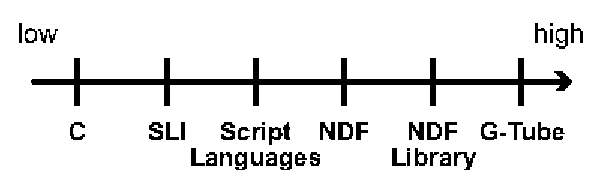
\includegraphics[width=4in]{figures/g3-interfacing.eps}
\end{center}
\caption{
{\bf Levels of programing in GENESIS 3.0.} The concept hierarchy used for communication by GENESIS developers. C Coding: System programing languages are used to program individual simulator components and extend simulator functionality. SLI: Indicates the level of the GENESIS-2 Script Language Interface in the concept hierarchy. Script Languages: Python and Perl are used to interface individual simulator components. NDF: The native declarative file format used to build models and model components. NDF Libraries: Model components such as membrane channels and synapses provide a library of functional components available for accelerated model development. G-Tube: The GENESIS graphical user interface allows users to access models and model components for the rapid development of single cell and network models.
}
\label{fig:g3-interfacing}
\end{figure}

\clearpage

Figure 2

\begin{figure}[ht]
\begin{center}
%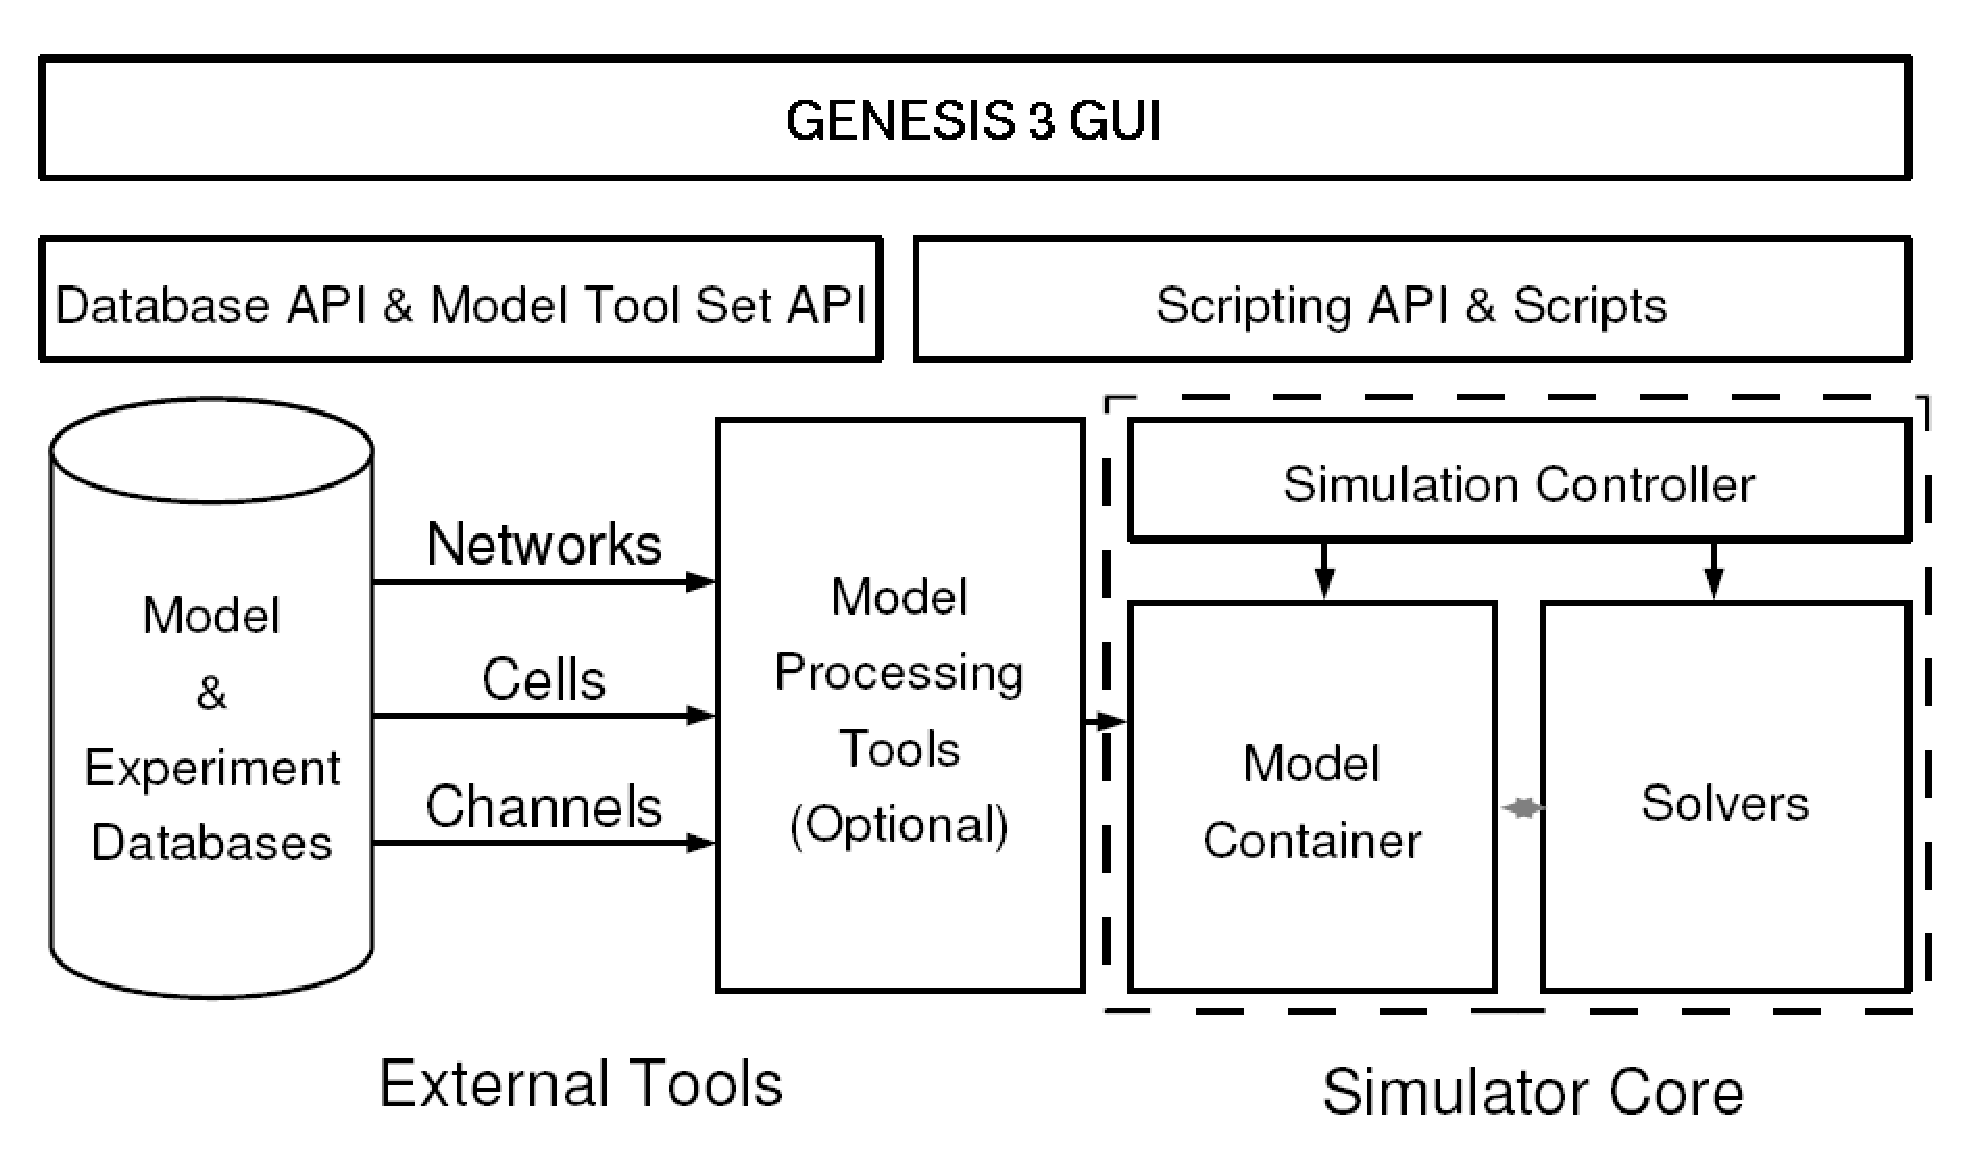
\includegraphics[width=4in]{figures/G3arch.eps}
\end{center}
\caption{
{\bf Relation of components in the Computational Biology Initiative (CBI) federated software architecture.} The CBI architecture defines the relationships between the necessary components of a computer-based neural simulation system. The architecture contains three layers that include a graphical user interface (GUI) connected to the functional components of a simulator by an interposed layer of application programming interfaces (APIs) and scripts. Components in the lowest layer are interconnected by APIs while their particular functionality is needed. GENESIS 3 is the first simulator to be implemented in compliance with the CBI architecture.
}
\label{fig:cbi-arch}
\end{figure}

\clearpage

Figure 3

\begin{figure}[ht]
\begin{center}
%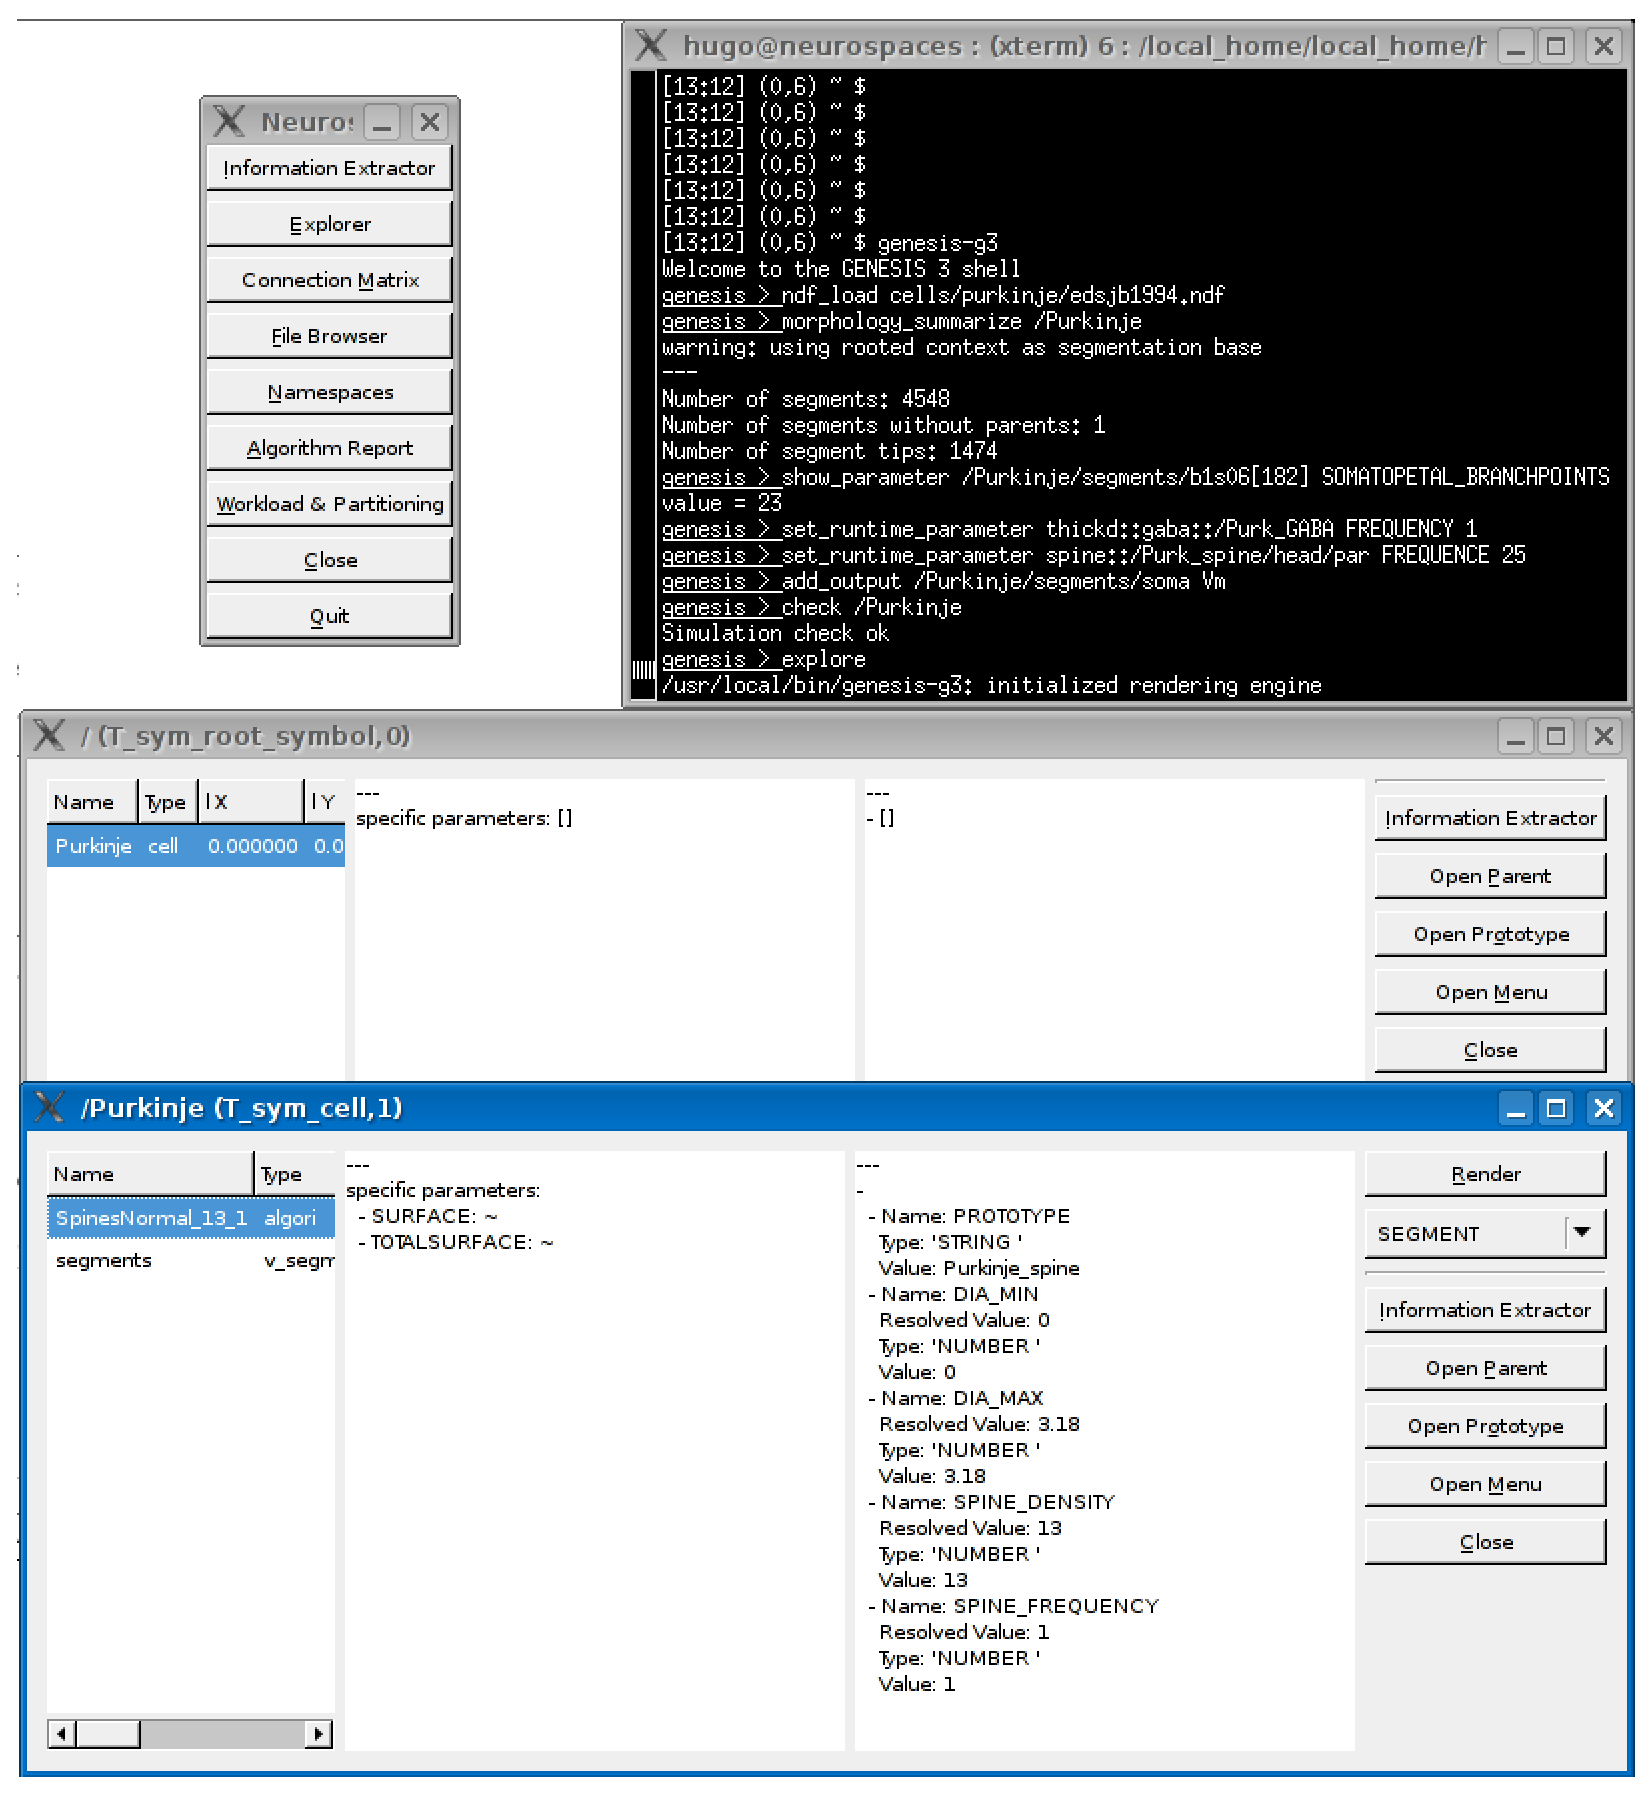
\includegraphics[width=4in]{figures/studio-screenshot.eps}
\end{center}
\caption{
{\bf Querying a model in GENESIS 3.0.} The {\bf Studio} is a component of the reconfigured GENESIS software platform. It can be used to query the parameters of individual compartments in a multi-compartment model neuron. The {\bf Studio} also renders 3D morphology of dendrites and generates overviews of network models.
}
\label{fig:cbi-studio}
\end{figure}

\clearpage

Figure 4

\begin{figure}[ht]
\begin{center}
%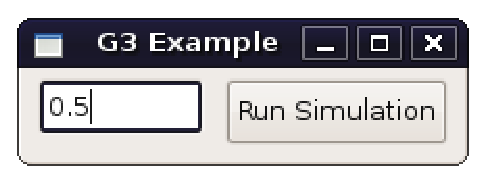
\includegraphics[width=2in]{figures/Screenshot-G3-Example.eps}
%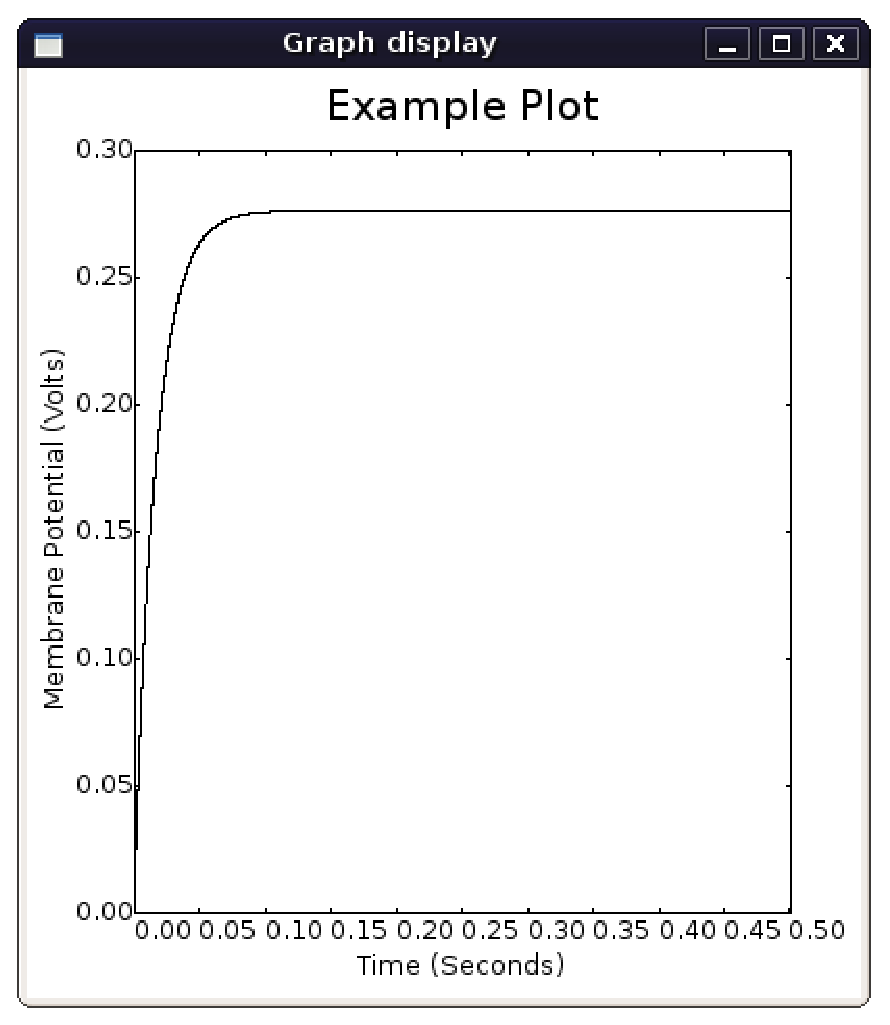
\includegraphics[width=4in]{figures/Screenshot-Graph-display.eps}
\end{center}
\caption{ {\bf Simple Integration of G-3 with the {\it wxPython}
    widget set.}  The CBI architecture defines a separation between
  GUI statements and peripheral code.  This allows GUI construction
  kits to be used for the creation of a user-friendly interface to a
  simulation.  In this example {\it wxFormBuilder} was used to
  construct a text control widget and a button to start the simulation
  using its standard drag \& drop interface.  The same approach can be
  used for the development of research and educational projects.  }
\label{fig:g3-wx}
\end{figure}

\clearpage

Figure 5

\begin{figure}[ht]
\begin{center}
%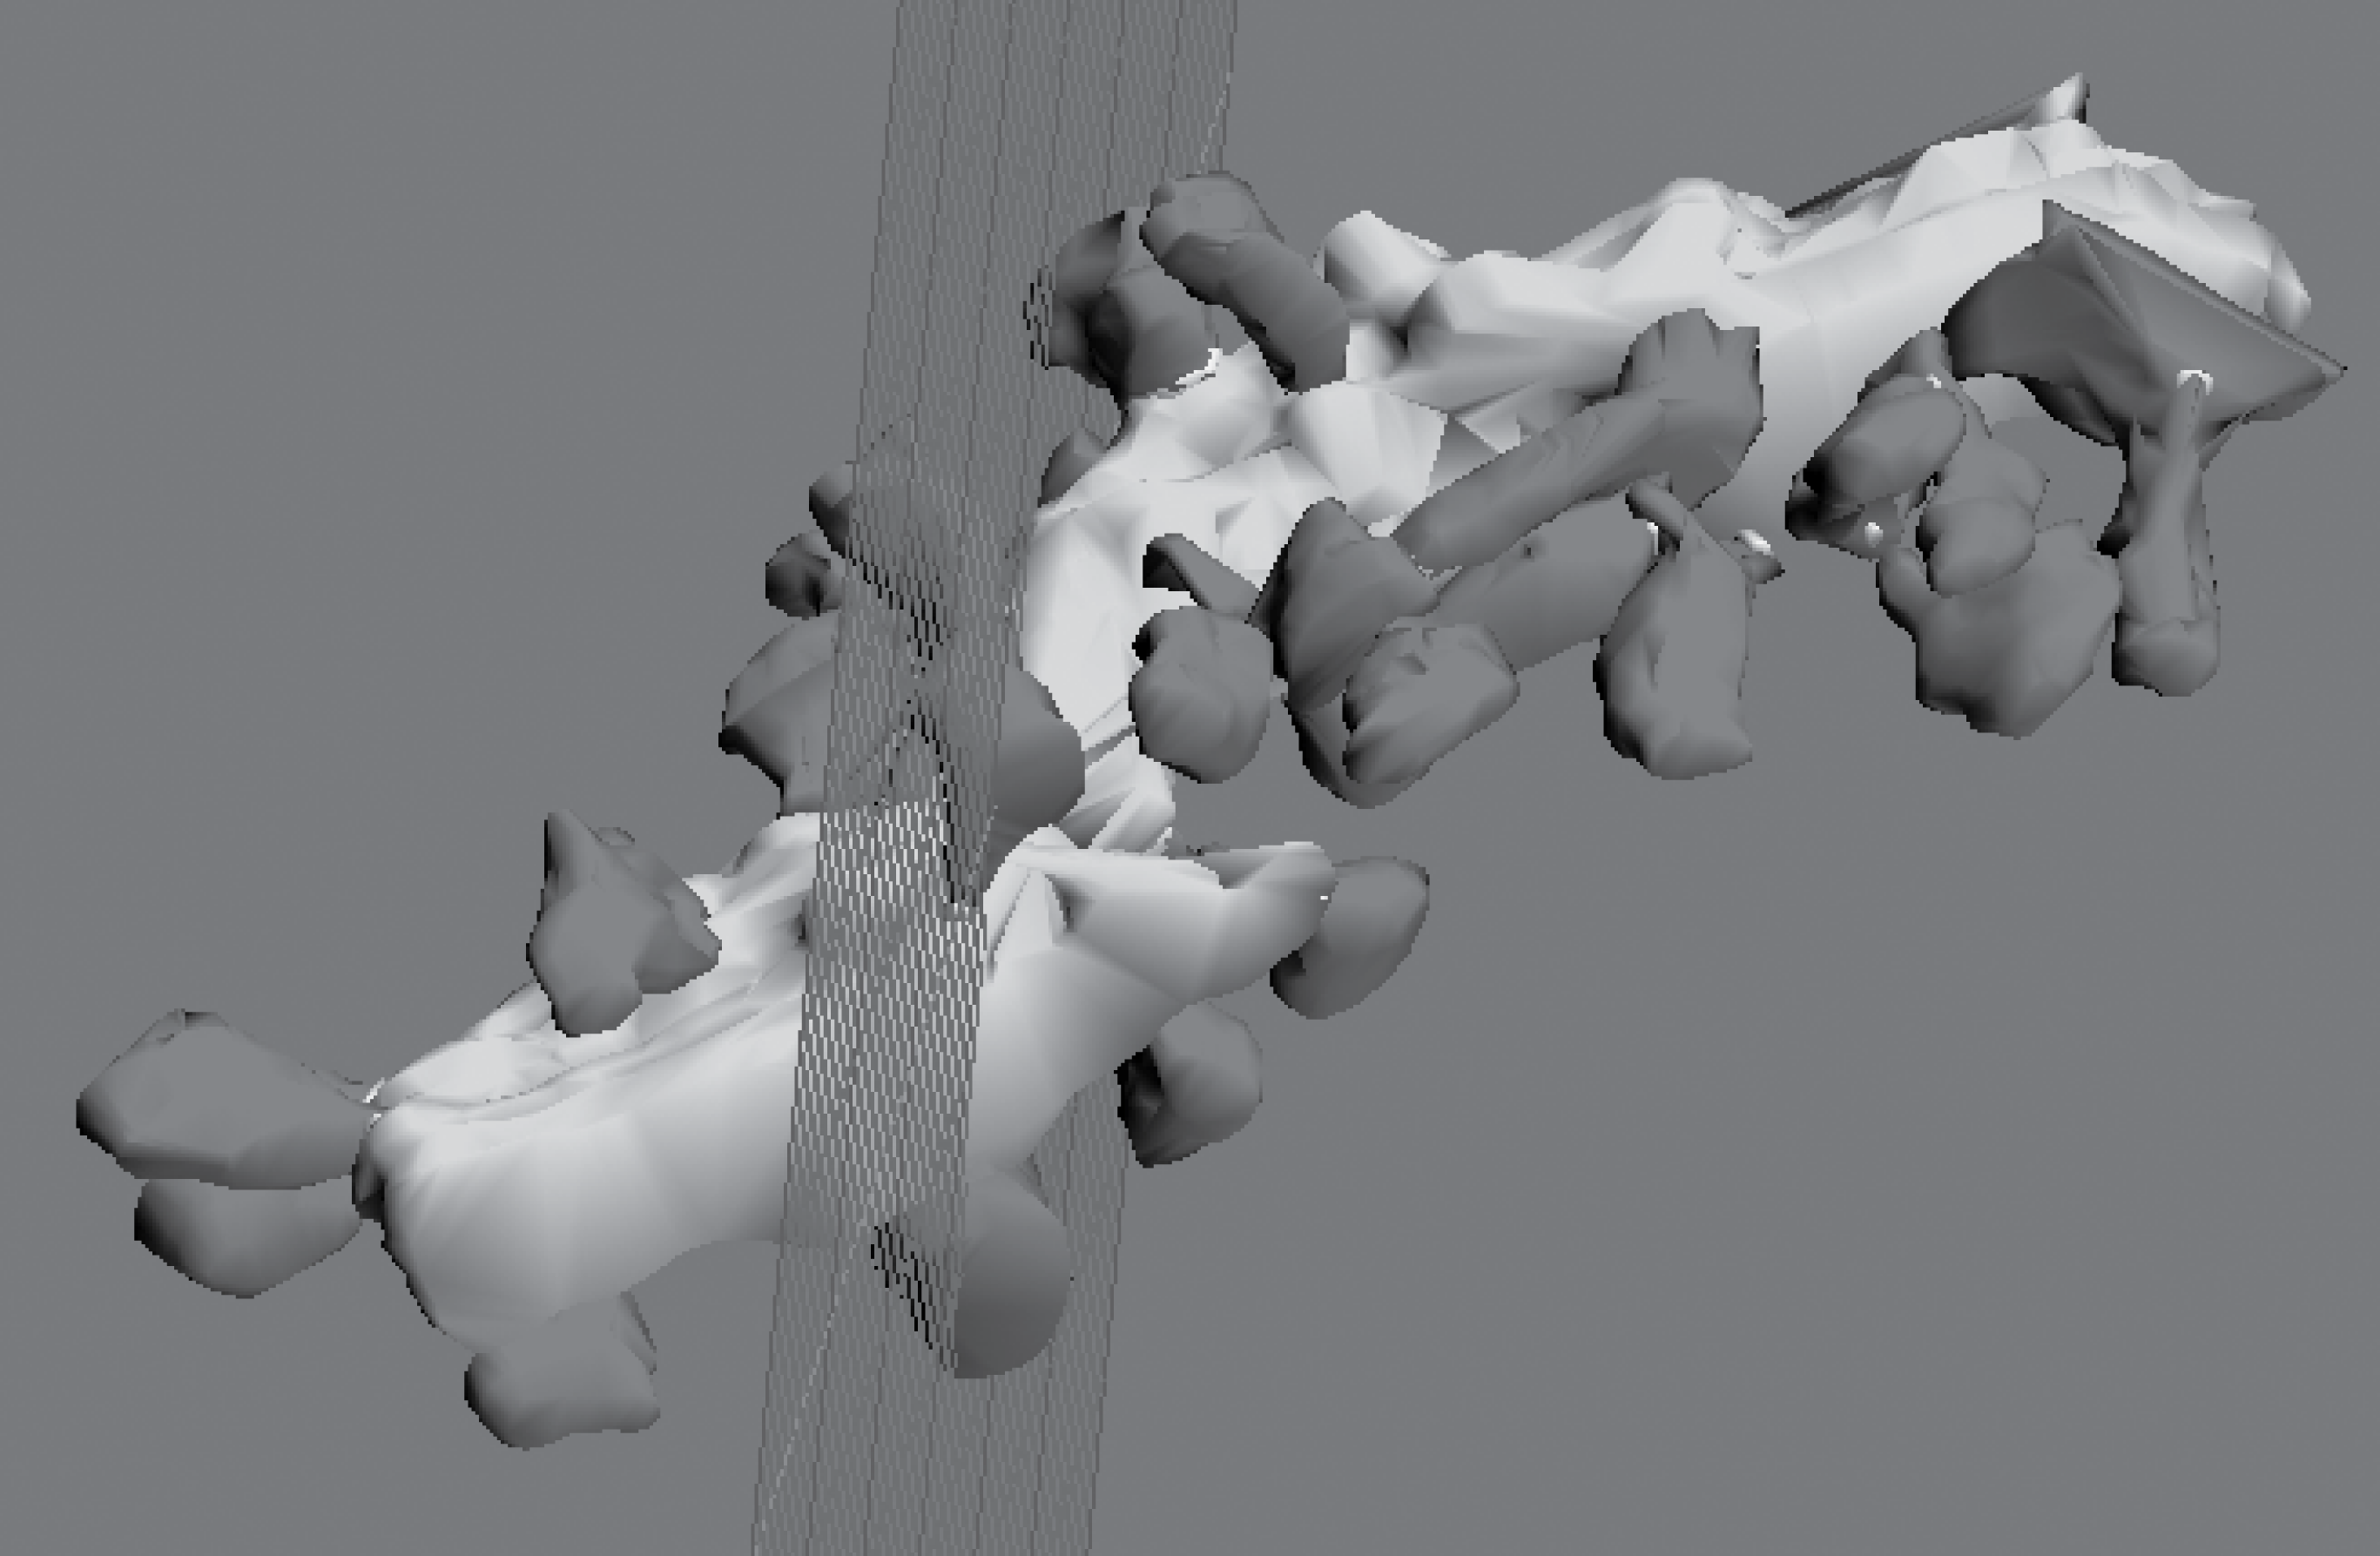
\includegraphics[width=4in]{figures/blender-python-bw.eps}
\end{center}
\caption{
{\bf Image of reconstructed Purkinje neuron dendritic segment.} Blender is an open source 3D content creation suite that can be interfaced with the GENESIS neural simulation platform to replace the functionality otherwise provided by the {\bf G-Shell} (a stand-alone GENESIS component). The rendering functions of Blender can then be used to analyze the morphology of small dendritic segments imported from electron microscopy data.
}
\label{fig:cbi-blender}
\end{figure}

\clearpage

Table 1

%
%%\section*{Tables}
%%\begin{table}[!ht]
%%\caption{
%%\bf{Table title}}
%%\begin{tabular}{|c|c|c|}
%%table information
%%\end{tabular}
%%\begin{flushleft}Table caption
%%\end{flushleft}
%%\label{tab:label}
%% \end{table}
%
\begin{table}[ht]
\caption{
\bf{Comparison of Hand-Written and Generated Code (in Byte Counts).}}
%\begin{tabular}{l c c c c c c}

%    {\bf Language:}
%    & {\bf C (H)}
%    & {\bf C (G)}
%    & {\bf Perl (H)}
%    & {\bf Perl (G)}
%    & {\bf Python (H)}
%    & {\bf Python (G)} \\

%    {\bf Model Container}
%    & 1,832,580
%    & 4,416,163
%    & 30,406
%    & 207,638
%    & 14,568
%    & 250,178 \\

%    {\bf Heccer}
%    & 1,163,991
%    & 1,575,615
%    & 57,565
%    & 107,261
%    & 1,586
%    & 171,219 \\

%    {\bf NS-SLI}
%    & 1,448,636
%    & 483,641
%    & 4,603
%    & 2,802
%    & ---
%    & --- \\

%    {\bf SSP}
%    & 829
%    & 2,323
%    & 55,063
%    & ---
%    & ---
%    & --- \\

%    {\bf Studio}
%    & ---
%    & ---
%    & 174,923
%    & ---
%    & ---
%    & --- \\

%    {\bf G-Shell}
%    & ---
%    & ---
%    & 28,142
%    & ---
%    & 623
%    & 836 \\
%\end{tabular}
\begin{flushleft} A\marginnote{
  \begin{picture}(0,0)
    \put(-10,10){\line(0,-1){0}}
  \end{picture}
} comparison of hand-written (H) and automatically generated (G) code that supports the functionality of the independent components of the GENESIS simulation platform. Software hand-written in a system programming language such as C contains more code (in bytes) than the equivalent functionality replicated in a scripting language. The amount of automatically generated code is considerably greater than that written by hand.
\end{flushleft}
\label{tab:cbi-codecounts}
\end{table}

%\clearpage

%\begin{figure}[ht]
%\begin{center}
%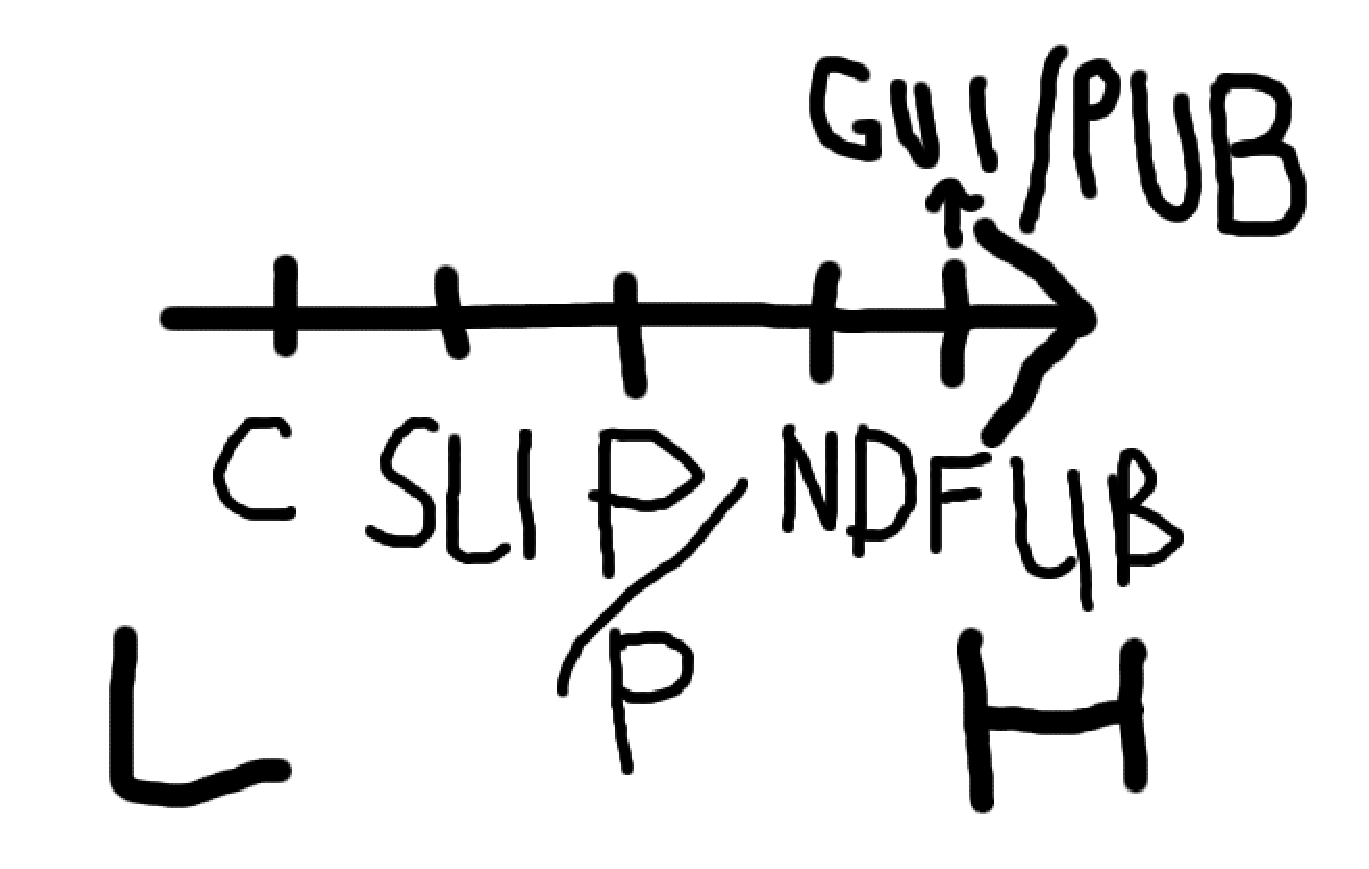
\includegraphics[width=4in]{figures/conceptual-hierarchy.eps}
%\end{center}
%\caption{
%{\bf Relationship Hierarchy between GENESIS Configurability and Extenxibility Options.}
%}
%\label{fig:conceptual-hierachy}
%\end{figure}


\end{document}
